%%%%%%%%%%%%%%%%%%%%%%%%%%%%%%%%%%%%%%%%%%%%%%%%%%%%%%%%%%%%%%%%%%%%%%%%%%%%%%%%
%2345678901234567890123456789012345678901234567890123456789012345678901234567890
%        1         2         3         4         5         6         7         8

\documentclass[letterpaper, 10 pt, conference]{ieeeconf}  % Comment this line out if you need a4paper

%\documentclass[a4paper, 10pt, conference]{ieeeconf}      % Use this line for a4 paper

\IEEEoverridecommandlockouts                              % This command is only needed if 
                                                          % you want to use the \thanks command

\overrideIEEEmargins                                      % Needed to meet printer requirements.

%In case you encounter the following error:
%Error 1010 The PDF file may be corrupt (unable to open PDF file) OR
%Error 1000 An error occurred while parsing a contents stream. Unable to analyze the PDF file.
%This is a known problem with pdfLaTeX conversion filter. The file cannot be opened with acrobat reader
%Please use one of the alternatives below to circumvent this error by uncommenting one or the other
%\pdfobjcompresslevel=0
%\pdfminorversion=4

% See the \addtolength command later in the file to balance the column lengths
% on the last page of the document

% The following packages can be found on http:\\www.ctan.org
%\usepackage{graphics} % for pdf, bitmapped graphics files
%\usepackage{epsfig} % for postscript graphics files
%\usepackage{mathptmx} % assumes new font selection scheme installed
%\usepackage{times} % assumes new font selection scheme installed
%\usepackage{amsmath} % assumes amsmath package installed
%\usepackage{amssymb}  % assumes amsmath package installed
\usepackage{graphicx}
\usepackage{epstopdf}
\usepackage{amsmath}
\usepackage{xcolor}
\usepackage{amssymb}
\usepackage{subfigure}
\usepackage{multirow}
\usepackage{pbox}
\usepackage{algorithm}
\usepackage{algorithmic}
\usepackage{cite}


%\usepackage{algpseudocode}
\usepackage{bm}
\usepackage{url}
\newcommand\NB[1]{$\spadesuit$\footnote{NB: #1}}


\newcommand{\R}{\mathbb{R}}
\newcommand{\Z}{\mathbb{Z}}
\newcommand{\D}{\mathbb{D}}
\newcommand{\N}{\mathbb{N}}

\newtheorem{problem}{Problem}
\newtheorem{lemma}{Lemma}

\DeclareMathOperator*{\argmin}{arg\,min}
\DeclareMathOperator*{\argmax}{arg\,max}

\begin{document}

\title{\LARGE \bf
Parameter-free Regression-based Autonomous Control of Off-the-shelf Quadrotor UAVs
}


\author{Rahul Peddi and Nicola Bezzo%
\thanks{Rahul Peddi and Nicola Bezzo are with the Department of Systems and Information Engineering and the Charles L. Brown Department of Electrical and Computer Engineering, University of Virginia, Charlottesville, VA 22904, USA. Email: {\tt \{rp3cy, nb6be\}@virginia.edu}}}



\maketitle
\thispagestyle{empty}
\pagestyle{empty}


%%%%%%%%%%%%%%%%%%%%%%%%%%%%%%%%%%%%%%%%%%%%%%%%%%%%%%%%%%%%%%%%%%%%%%%%%%%%%%%%
\begin{abstract}
Autonomous flight in unmanned aerial vehicles (UAVs) generally requires platform-specific knowledge of the dynamical parameters and control architecture. Recently, UAVs have become more accessible with off-the-shelf options that are well-tuned and stable for user teleoperation. In this paper, we develop a method to enable autonomous flight on vehicles that are designed for teleoperation with minimal knowledge of the dyanmical and controller parameters. The proposed method uses a basic knowledge of the control and dynamic architecture along with human teleoperated trajectories demonstrations to train a thin-plate spline (TPS) regression model, which is then used to manipulate the pre-trained commands to generate new autonomous input commands for autonomous navigation over new trajectories. A robust control-based strategy is also proposed to adjust autonomous input commands in real-time for closed loop trajectory tracking. Finally, we validate the proposed approach with trajectory-following experiments on a quadrotor UAV.

\end{abstract}


%%%%%%%%%%%%%%%%%%%%%%%%%%%%%%%%%%%%%%%%%%%%%%%%%%%%%%%%%%%%%%%%%%%%%%%%%%%%%%%%
\section{Introduction}
%\NB{Motivation here is that it is hard to generate autonomous flight because every platform is different and you need to show what's the typical iteration to generate autonomous flight with quadrotor based on model. Not using controller based on model - structure of model, but no specifics or parameters - not always available. By demonstrating we can extract a way to move the system}
Unmanned Aerial Vehicles (UAVs) have become widespread for both civilian and military applications in recent years. There are several applications for which UAVs are uniquely suited over other robotic systems, such as surveillance, delivery services, and search and rescue. All of these applications require the UAV to autonomously follow trajectories to different goal or task locations. For example, a package delivery UAV may have to autonomously reach multiple locations at certain times to deliver and receive new packages. 

The development of dedicated platforms for such autonomous tasks can be expensive and not necessary since hundreds of off-the-shelf UAVs are available nowadays and for low cost. These platforms are usually well designed, very stable, and ready to fly out of the box but are typically restricted to teleoperation usage.

Generating autonomous flight behavior - the subject of this paper -  however, can be difficult since every UAV has different dynamical parameters, which are typically not available, and reverse engineering is often not possible. Model-based approaches that include system identification, model extraction, and control design are well known procedures to deal with this issue however they are time demanding and often not precise requiring a lot of tuning and testing \cite{modelbased1}. Even when these approaches are successful, among similar vehicles there can be model mismatch due to manufacturing error, different usage, physical alterations, or aging which can change parameters thus needing more tuning or sophisticated adaptive control architectures to guarantee safe and reliable control. 
%While model driven procedures are time demanding, they
%, and knowledge of that model is required to generate autonomous flight. Extracting this model is time demanding

On the other hand, data-driven machine learning techniques like neural networks, reinforcement learning, and regression techniques have recently emerged and have demonstrated to be effective to learn from training data. The main drawbacks of such procedures is that there is still not a clear reasoning about how these techniques work and typically large and dense training sets are required to obtain precise results.
\begin{figure}[t]
    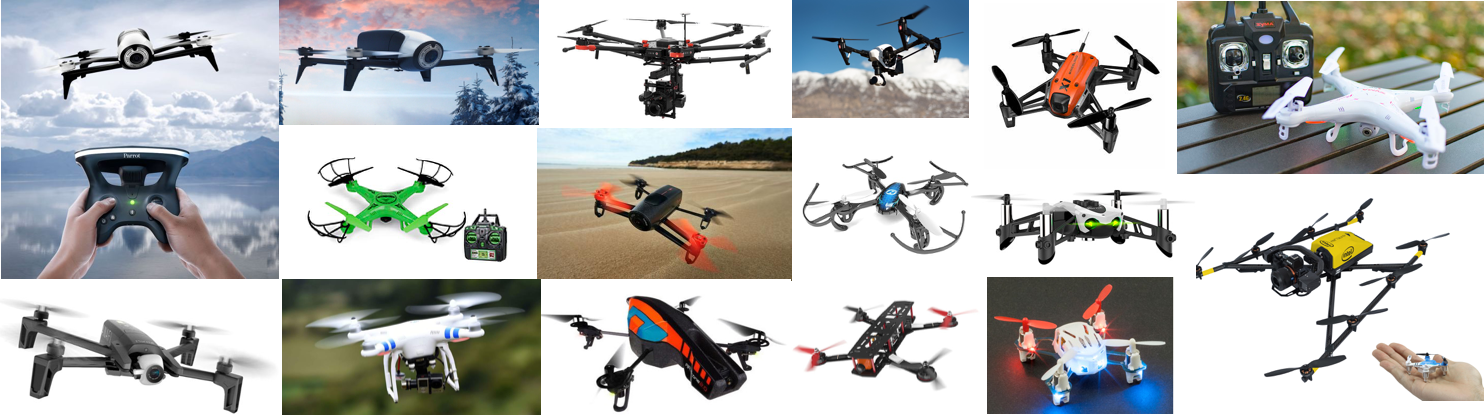
\includegraphics[width=0.48\textwidth]{images/quads.png}
    \vspace{-5pt}
    \caption{Some Examples of Off-the-Shelf UAVs, courtesy of the web}
    \label{fig:uavs}
    \vspace{-15pt}
\end{figure}
\NB{I've changed the figure. We need also one that show what we are doing here. I'll help with the figures}
Different from other supervised learning approaches, in this work we leverage the knowledge about the generalized architecture for the UAV dynamics and their controller and use regression-based techniques to extract a model for closed loop trajectory tracking. The main contribution of this work is a framework that combines both model-based and data-driven theories to generate autonomous control for aerial vehicles. We also provide a framework to assess the quality of the training data with an error analysis of our regression model that impacts decisions we make in terms of UAV trajectory and autonomous control generation.
In this work we propose a novel approach that leverages both model-based and data-driven theories to generate autonomous flight behavior for an aerial vehicle from few user teleoperation demonstrations. 
We focus on off-the-shelf quadrotor UAVs which have a well studied dynamical and control architecture and are by far the most common UAVs because of the growing hobby and DIY community. Even if the application focus of this paper is on quadrotors, our framework can scale and apply to any other teleoperated aerial vehicle. Fig. \ref{fig:uavs} shows some examples of such quadrotors focus of this paper, all characterized by having the same shape but different motors, propellers, boom size, and electronics and hence different dynamic and control models.



The remainder of the paper is organized as follows: In Section \ref{sec:relatedwork}, we present the state of the art in the literature. In Section \ref{sec:prob}, we formulate our problem statement. In Section \ref{sec:sysdyn}, we discuss the system dynamics and controller architecture, which is then followed by an overview of our methodology in Section \ref{sec:approach}. Finally, we end with a discussion about our experimental validation in Section \ref{sec:exper}, and we have our conclusions and a discussion on future work in Section \ref{sec:conc}.

%We then discuss in detail each part of our approach with training in Section \ref{sec:train}, trajectory generation in Section \ref{sec:traj}, autonomous control generation in Section \ref{sec:generate}, and lastly the online adaptation of controls in Section \ref{sec:adapt}.
%\NB{no need to list all subsections just list teh main section details}
%Besides a general framework for the generation of autonomous commands for any quadrotor, in this work we offer a scheme to integrate model-based and data-driven approaches 
%\NB{need to reinforce this statement}
 
%In order to address these challenges, our approach leverages the generalized dynamics of UAVs along with regression analysis on demonstrations and elements of control theory to generate autonomous flight and ensure that the vehicle can track any trajectory. 
 
% and correction to minimize tracking error.
%architecture (note that parameters are unknown)
%extracting the rule for open loop trajectory tracking and correcting to minimize tracking error


%here the vehicle doesn't only repeat what the user is teaching and the training set can be smaller because knowledge bout the system model is used to guide the input generation.

%Both model-based and data-driven theories are leveraged to  


%Traditionally, autonomous control of UAVs consists of four control inputs: thrust, roll, pitch, and yaw. For these control inputs to actually create motion, knowledge about the physical system (e.g., mass and moments of inertia) is required [CITE]. This information, however, can vary quite a lot for different systems [show image of two very different uavs here], and the specifics and parameters of the dynamic models are not always available.
%
%This need for platform-specific parameters, however, can be avoided if we can learn what control inputs to send to the vehicle in another way. The parameters are generally only necessary when generating autonomous flight, but when there is a human pilot, the controls are sent to the system in a different manner, usually via teleoperation commands. In this work, we are interested in transferring this knowledge from a human-piloted demonstrations for fast learning and generation of autonomous flight, all while being unaware of platform-specific parameters. It is, however, trivial to replicate the actions of the human pilot to generate the same action autonomously. As a result, we are interested in taking a library of a several demonstrations to enable the vehicle to follow any generated trajectory.
%
%To this end, we propose a framework that aim the solve the following challenges:
%\begin{itemize}
%    \item how to enable autonomous flight in aerial vehicles with minimal knowledge of vehicle dynamics
%    \item how to learn to correct 
%%    \item how to expand the knowledge obtained from several demonstrations to follow any trajectory
%\end{itemize}

%\NB{we need to stress that these quadrotors already come with well designed controllers and at the bare minimum we can teleop}

%The rest of this paper is organized as follows: In Section \ref{sec:traj}, we discuss how we generate and decompose smooth trajectories for our UAV to follow. Next, we discuss the training data and regression analysis in Section \ref{sec:train}. This is then followed by discussing how the autonomous commands are generated in Section \ref{sec:generate}, which is followed by the online adaptation and correction in Section \ref{sec:adapt}. Lastly, we describe and demonstrate our experimental results in Section \ref{sec:exper}, and we conclude our work and discuss future work in \ref{sec:conc}.

\section{Related Work} \label{sec:relatedwork}
%\NB{we need to stress how different this work is in comparison with the rest of the literature on learning from demonstration. We need to show our contribution clearly}
\NB{skipping related work for now}

In recent years, we have had many advancements in unmanned aerial vehicles (UAVs). A very common and widely researched task for UAVs is motion and path planning. The authors in \cite{minsnap,waypts,tvec} provide well optimized approaches for UAV trajectory generation and tracking by utilizing near perfect knowledge of the controller and dynamical model parameters. Access to these parameters, as they are in our case, are often limited. In \cite{pso}, the authors leverage exact knowledge of the model dynamics an controller architecture to identify necessary parameters for trajectory tracking, and perform parameter estimation using particle swarm optimization, which can be a long and iterative process, which is the case for many other model-based parameter and system identification approaches \cite{modelbased1,modelbased2}.

Some of the more recent advancements in this area feature machine learning and data-driven approaches, such as deep learning (DL), imitation learning (IL), and reinforcement learning (RL). In \cite{dln}, the authors use DL to learn driving models for ground vehicles by using large-scale video datasets, and in \cite{rlctrl}, the authors use RL over $1,000$ training samples for accurate quadrotor trajectory tracking. These methods are model and parameter free, but use extremely large datasets to resolve that issue. In \cite{uavrace}, the authors explore the idea of observational imitation learning (OIL), where learning is achieved from a relatively small number of demonstrations, but knowledge of the controller architecture is assumed and parameter estimation is performed, which can be a daunting task without knowledge of the controller architecture. The authors in \cite{abbeel} use apprenticeship learning, which is similar to IL, to train a UAV to perform trajectories with a very simplified model, but there is still a necessity to learn some dynamical parameters, while assuming knowledge of several others, such as mass and moments of inertia. Despite having to learn certain parameters, the same authors show the ability to learn some maneuvers using only important information from only $20$ minutes of flight time, however, it is an episodic task and takes a significant amount of testing for convergence. The understated desire for smaller training sets is prevalent in many of the works in this area. Some works, such as \cite{gppaper} use a stochastic method known as a Gaussian Process (GP) to accurately tune a simplified UAV controller. Use of stochastic or regression based methods, such as GPs have shown the ability to execute imitation learning with limited training sets and information \cite{imlerngp,imlernreg}.

Our work leverages knowledge about the system dynamics architecture combined with regression theory to learn to fly autonomously aerial vehicles.
% abut not the paprametrsis largely based on combining the aforementioned apprenticeship learning theory with a regression method - we show how we can obtain and analyze important information from a relatively small number of demonstrations. 
Contrary to most model based approaches, we assume no knowledge of specific dynamical parameters, while only knowing the structure of the dynamical model and controller architecture. 
%This makes parameter estimation a rather unfeasible and inefficient task. 
Instead of estimating parameters, we use information obtained from human-piloted training demonstrations to directly generate control inputs to track a trajectory, by way of training and analyzing a regression model and implementing online corrections.


%\NB{overall outline for reference: model of quadrotor is unknown but skeleton architecture is known and the controller is u1, u2, u3 = equations. Because of how the controller is designed, we know that u2 is used to change x and u3 y. A change in u2 is equivalent to a change in the x position. The higher is this change the more motion is generated hence the area under the curve described by the commands sent to the quadrotor is related to the motion of the system and here is where the regression approach is sued. Instead of learnign the parameters that is hard we use regression to learn to fly directly by leveraging the integral and the knowledge about the system. }

\section{Problem Formulation} \label{sec:prob}
In this work, we are interested in developing autonomous navigation for a UAV by leveraging knowledge about its system dynamics and controller along with a set of human-piloted demonstrations.
%in using human-piloted demonstrations to develop a framework that enables autonomous UAV navigation over any trajectory with minimal knowledge of platform-specific dynamics.
Formally, the problem we investigate in this work can be stated as:

\begin{problem}
 \textbf{\textit{Parameter-free Autonomous Control of UAVs}}: 
Consider a pre-configured off-the shelf ready to fly UAV, with known model architecture $\dot{\bm{x}}=f(\bm{x},\bm{u})$ where $\bm{x}$ is the state and with input $\bm{u}=g(\bm{x})$ and unknown internal parameters $\mathcal{P}$. Design a policy to generate the sequence of inputs $\bm{u}$ to track a user defined reference trajectory $\bm{x}_r(t),~ t \in [0,T]$ over a finite horizon $T$. Specifically the policy should ensure that the UAV position $\bm{p}(t)$ is always within a certain threshold $\delta_d$ from the generated trajectory position $\bm{p}_r(t)$
 \begin{equation} \label{eq:positlive}
        ||\bm{p}(t)-\bm{p}_r(t)|| \leq \delta_d,~\forall t \in [0,T]
    \end{equation}
    where $||\cdot||$ is the Euclidean norm.
\end{problem}
%    where $\bm{p_r}(t)$ is the reference position at time $t$, where $T$ represents an overall time horizon for the trajectory, and $\delta_d$ is a threshold for allowable deviation.
%A UAV has the objective to track a trajectory $\bm{p_r}(t),~ t \in [0,T]$ without specific knowledge of its model parameters
%
%visit a set of $n$ goals, $\bm{g}\in\mathbb{R}^{n}$, at a set of $n$ target times, $\bm{t} \in\mathbb{R}^{n}$. Given $m$ human-piloted flight demonstrations, the aim is to find a policy that enables autonomous flight to generate and track a trajectory $\bm{p_r}(t),~ t \in [0,T]$ that visits the target goals $\bm{g}_i$ at the respective target times, $\bm{t}_i$, such that the following liveness requirements are met:
%\begin{enumerate}
%    \item  Position: The UAV should always stay within a certain distance of the generated trajectory:
%    \begin{equation} \label{eq:positlive}
%        ||\bm{p}(t)-\bm{p_r}(t)|| \leq \delta_d,~\forall t \in [0,T]
%    \end{equation}
%    where $\bm{p_r}(t)$ is the reference position at time $t$, where $T$ represents an overall time horizon for the trajectory, and $\delta_d$ is a threshold for allowable deviation.
%    \item  Time: The UAV should always reach the target locations within a certain threshold of the target time for that goal:
%    \begin{align}
%        \tau = t\in[0,T]|\bm{p}(t)-\bm{g}_i \leq \delta_d \nonumber \\
%        |\tau- \bm{t}_i| \leq \delta_t,~i=1,\ldots,n \label{eq:time_live}
%    \end{align}
%    where $\tau$ is a time at which the liveness condition is met for a specific goal and $\delta_t$ is the allowable deviation in time from the target.
%\end{enumerate}
\section{System Models} \label{sec:sysdyn}
%\NB{in this section we need to show the dynamical model, and control model and architecture with teleoperation. We need to stress that everything is a gray box with known model but unknown params and that the inputs and outputs are known and used later to obtain a model for autonomous fly. We need to explain the relation between teleop and u1 u2 u3 and u4 and how increasing the joystick increase the inputs and thus the integral measures mobility in the system.}
As hinted in the introduction, we use knowledge about the UAV dynamics and control architecture to extract useful information about the system to guide a regression approach for the generation of autonomous control commands for the UAV. We focus on off-the-shelf tuned and stable quadrotors that typically are ready for teleoperation but not for autonomous flight. The control architecture of the off-the-shelf quadrotor is shown in Fig.~\ref{fig:otsctrl}.
\begin{figure}[ht]
    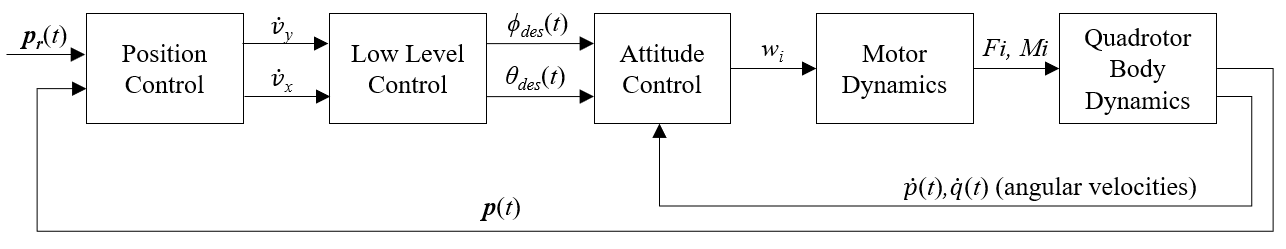
\includegraphics[width=0.48\textwidth]{images/ctrler.png}
    \caption{Off-the-Shelf UAV Teleoperation Control Architecture}
    \label{fig:otsctrl}
\end{figure}
%\NB{this figure is too small...text need to be bigger}
The presented structure is a gray box model, where the only information known are the teleoperation inputs, indicated by $\bm{J}_x$ and $\bm{J}_y$, the output, which is the position of the vehicle, $\bm{p}(t)$, over time, and the basic model architecture. The low level controller usually consists of multiple PID loops \cite{esen}, which are already developed and tuned with certain specific control gains, which can be very difficult to identify by analyzing the output of the system. The quadrotor body dynamics can be modeled using a $12^{\text{th}}$ order state vector as follows:
%\NB{why q in $\bm{p}_q$? In the problem formulation there is not q}
\begin{equation}
    \bm{q} = 
    \begin{bmatrix}
    \bm{p}^\intercal & \phi & \theta & \psi & v_x & v_y & v_z & \omega_x & \omega_y & \omega_z
    \end{bmatrix}^\intercal \nonumber
\end{equation} 
%\NB{use $\bm{p}_q$}
where $\bm{p}=[x \; y \; z]^{\mathsf{T}}$ is the world frame position, $v_{x}$, $v_{y}$ and $v_z$ are the world frame velocities, $\phi$, $\theta$ and $\psi$ are the roll, pitch and yaw Euler angles and $\omega_{x}$, $\omega_{y}$ and $\omega_{z}$ are the body frame angular velocities.

The dynamics of the vehicle are then described as follows \cite{esencite}:
\begin{equation} \label{eq:quadrotor_dynamics} 
	\begin{aligned}
	%\begin{bmatrix}\dot{x} \\ \dot{y} \\ \dot{z} \end{bmatrix} &= \begin{bmatrix}v_x \\ v_y \\ v_z\end{bmatrix}\\
	\dot{\bm{p}}^{\mathsf{T}} &= \begin{bmatrix}v_x & v_y & v_z\end{bmatrix}\\
	\begin{bmatrix}\dot{v}_x \\ \dot{v}_y \\ \dot{v}_z\end{bmatrix} &= \begin{bmatrix}0 \\ 0 \\ -g \end{bmatrix} + \frac{1}{m} \begin{bmatrix}\cos\phi \cos\psi \sin\theta + \sin\phi \sin\psi \\ \cos\phi \sin\theta \sin\psi - \cos\psi \sin\phi \\ \cos\theta \cos\phi \end{bmatrix} u_1\\
	%\end{align*}
	%\begin{align*}
	\begin{bmatrix}\dot{\phi} \\ \dot{\theta} \\ \dot{\psi}\end{bmatrix} &= \begin{bmatrix}1 & \sin\phi \tan\theta & \cos\phi \tan\theta\\ 0 & \cos\phi & -\sin\phi \\ 0 & \sin\phi \sec\theta & \cos\phi \sec\theta \end{bmatrix} \begin{bmatrix}\omega_{x} \\ \omega_{y} \\ \omega_{z} \end{bmatrix}\\
	\begin{bmatrix}\dot{\omega}_{x} \\ \dot{\omega}_{y} \\ \dot{\omega}_{z}\end{bmatrix} &= \begin{bmatrix}\frac{I_{yy} - I_{zz}}{I_{xx}} \omega_{y}\omega_{z}\\ \frac{I_{zz} - I_{xx}}{I_{yy}} \omega_{x}\omega_{z} \\ \frac{I_{xx} - I_{yy}}{I_{zz}} \omega_{x}\omega_{y} \end{bmatrix} +  \begin{bmatrix}\frac{1}{I_{xx}} & 0 & 0\\ 0 & \frac{1}{I_{yy}} & 0\\ 0 & 0 & \frac{1}{I_{zz}}\end{bmatrix} \begin{bmatrix}u_{2} \\ u_{3} \\ u_{4} \end{bmatrix}
	\end{aligned}
\end{equation} 

This dynamical model consists of many platform-specific parameters that are also difficult to identify, much like the controller gains discussed above. Moreover, these parameters often vary a lot between UAVs, and that further complicates the identification problem. The model and architecture above assume that the quadrotor is moving at a constant $z$ level with a zero yaw constraint, and therefore, we are primarily concerned with two of the inputs, $u_2$ and $u_3$. The equations for these two control inputs are as follows:
\begin{align} \label{eq:cinputs}
    %u_1 &= m(g + \ddot{z}_{des} + k_{d,z}(\dot{z}_{des}  \dot{z}) + k_{p,z}(z_{des}-z)) \nonumber \\
    u_2 &= k_{p,\phi}(\phi_c-\phi) + k_{d,\phi}(\dot{\phi}_c - \dot{\phi}) \nonumber \\
    \phi_c &= -\frac{1}{g}(\ddot{x}_{des} + k_{d,x}(\dot{x}_{des}-\dot{x}) + k_{p,x}(x_{des}-x)) \nonumber \\
    u_3 &= k_{p,\theta}(\theta_c-\theta) + k_{d,\theta}(\dot{\theta}_c - \dot{\theta}) \nonumber \\
    \theta_c &= -\frac{1}{g}(\ddot{y}_{des} + k_{d,y}(\dot{y}_{des}-\dot{y}) + k_{p,y}(y_{des}-y))
\end{align}
where $\phi_c$ and $\theta_c$ are the desired roll and pitch angles, respectively.

In this work, the goal is to generate control inputs for autonomous flight when the only information available for training comes from human-piloted demonstrations. Given these user demonstrations, we assume that the inputs and outputs for the UAV are visible, i.e., we can obtain position and velocity of the system during training as well as the input commands sent to the vehicles from the user teleoperation. 
%\NB{this part needs to be rewritten and generalized. We can mention later that in our case we use a MOCAP but here we just need to say that we assume that we can obtain position and velocity of the system during training as well as the commands sent to the vehicles as a result of the user teleop}
%\NB{this is also not true...we are not interested in learning from user. We are levergaing user teleop because it't the only thing we have and we are interested in generating commands for autonomous flight}

%Through observation of a single demonstrated trial, we are able to identify important commands sent to the system. 
%An example of such a trial is shown in Fig.\ref{fig:sampleintegral}. %\NB{this what? We cannot use this without any object on papers} is shown below \NB{avoid below above...they are vague...specify the figure number}:


%\NB{figures go after the explanation in the text}
%\NB{make these figures long and short and aligned vertically }
%\NB{we should show this picture in parallel with the speed and position of the vehicle to connect with the integral}
In Fig. \ref{fig:samps}, we show data from a single flight demonstration on a Parrot BeBop 2 quadrotor -- the hobby-grade quadrotor used in this paper to verify our results. The UAV was teleoperated forward manually over a distance of approximately $3$ meters, with initial and final velocities of $0$. The teleoperation input command string, in this case, corresponds to pitch, where a command of $0$ would imply no pitch adjustment, and $1$ corresponds to the UAV's maximum allowable pitch. The minimum allowable pitch command is $-1$, which flies the UAV in the negative $y$-direction. The teleoperation command, in this case, adheres to desired pitch angles, but the user could be adjusting any value that affects motion of the system, such as acceleration, torque, or even voltage provided to the motors depending on the factory setting. The approach presented in this paper is able to connect any of these commands to the change in position and velocity of the system.
\begin{figure}[ht]
	\centering
	\subfigure[Sample of a Single Demonstration\label{fig:sampleintegral}]{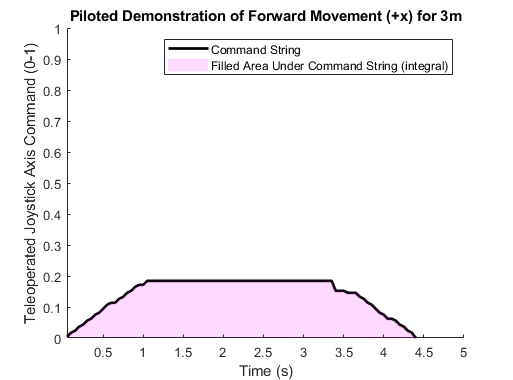
\includegraphics[width=1\linewidth]{images/sampleintegral.png}}
	\subfigure[Sample Distance Traveled\label{fig:sampt}]{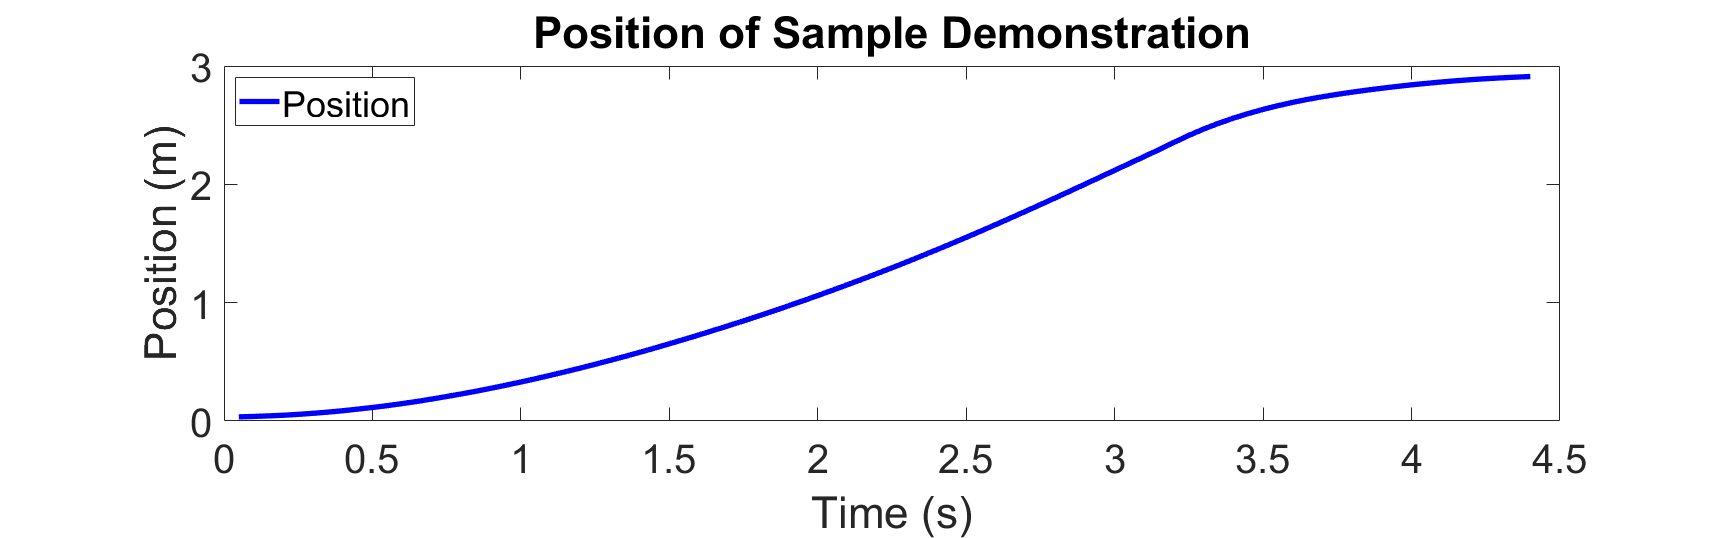
\includegraphics[width=1\linewidth]{images/sampletrajectory.png}}
	\subfigure[Sample Velocity\label{fig:sampv}]{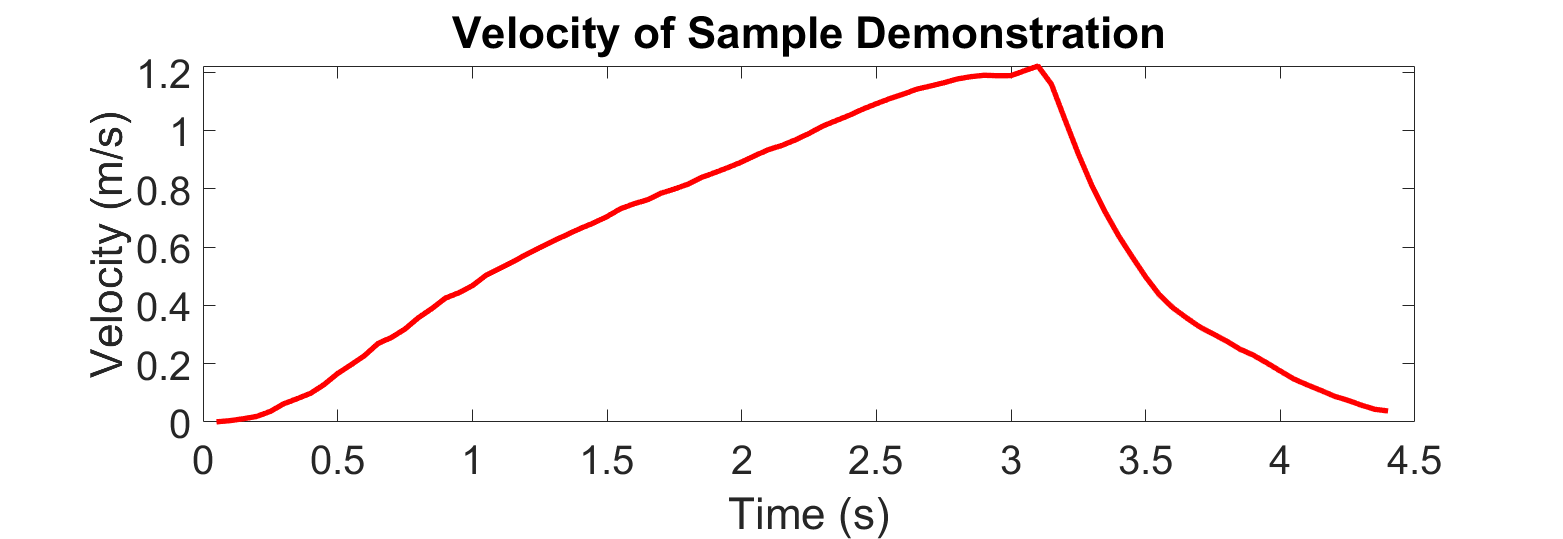
\includegraphics[width=1\linewidth]{images/samplevelocity.png}}
	\caption{Sample Demonstration, Distance Traveled, and Velocity}
	\label{fig:samps}
\end{figure}
From \eqref{eq:cinputs}, we observe that the inputs $u_2$ and $u_3$ for roll and pitch rely on the change in the desired Euler roll, $\phi_c$, and pitch, $\theta_c$, angles, and these desired roll and pitch angles are a function of the desired positions and velocities which are provided by the user, in our case. 
Hence, each stroke in the joystick transforms into motion of the vehicle which, in turn, affects its changes in the global $x$ and $y$ position. Our first goal here is to understand this mapping between user inputs and distance traveled by the quadrotor to build an autonomous behavior. Instead of using the entire string of commands, which could be large, not uniform, and computationally expensive, in this work we use the integral of the commands, in other words, the area underneath the time series of commands which is a compact and representative measure for training a model. The shaded area in Fig.~\ref{fig:sampleintegral} represents this integral. 

%In order to capture that that change in the desired angles, which are set by the human teleoperation, we take the area under the curve of the input commands. The shaded portion of Fig.\ref{fig:sampleintegral} represents this integral. Since these changes in roll and pitch affect the global $x$ and $y$ position of the vehicle, the integral that captures these changes is connected to the distance travelled by the vehicle. This integral is used as a compact measure for our training, and this removes the necessity to train on the entire string of commands, which could be large and more computationally intensive. 
%Along with the string of commands sent, the shaded portion of Fig.\ref{fig:sampleintegral}, represents the integral. i.e. the total area, under the string of commands. Because the pitch is proportional to the linear velocity in the $y$-direction, we know that the command string is proportional to the velocity, and its integral, therefore, is proportional to the distance traveled 
%\NB{here show that because u2 depends on $\phi_c$ and $\phi_c$ depends on x then this integral represents motion but what you really need to stress is that it is a compact measure without having to use the entire string of commands for learning}.

Because the integral by itself may not be enough to characterize a unique behavior of the UAV, as the same integral can be achieved with commands strings for different traveling distances and velocities, the average input command is also of interest since \eqref{eq:cinputs} impacts changes in traveling velocity in \eqref{eq:quadrotor_dynamics}. By using the combination of integral and average input commands, we will present an approach to generate autonomous commands during a mission defined by traveling through multiple waypoints at specified distances and times.

\section{Methodology} \label{sec:approach}
\begin{figure}[ht]
    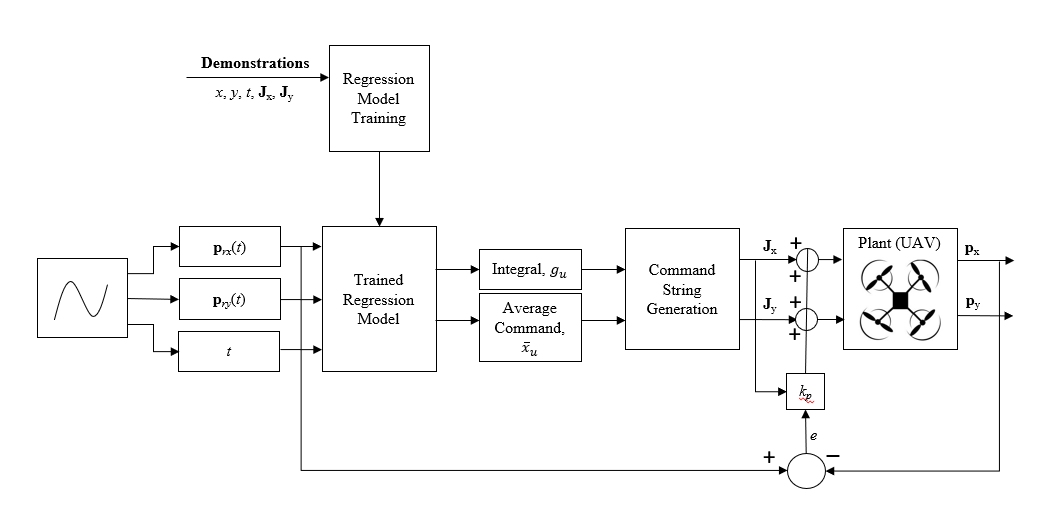
\includegraphics[width=0.48\textwidth]{images/blocks.PNG}
    \caption{Block Diagram of Proposed Approach}
    \label{fig:blockdiagram}
\end{figure}
%\NB{the figure needs to be changed. jx(t) jy(t) should input into the plant and the output is x(t) y(t) and all goes as input to the Training. The figure is still blurry}
%\NB{let's use power point fro the diagrams..it's blurry}
Our approach, outlined in Fig.~\ref{fig:blockdiagram}, consists of a training phase with multiple demonstrations that are used to build a regression model to identify the desired integral of the input commands, $g_u$, and desired average teleoperation input command, $\bar{j}_u$, from which a sequence of commands are synthesized to track a user-defined distance, $d_u$, in a time, $t_u$. The overall output of the regression is a sequence of commands having the same form of the inputs used for training which in our case are joystick teleoperation commands $\mathbf{J}_x(t)$ and $\mathbf{J}_y(t)$, needed by the system to follow the given trajectory. These actions are, however, open-loop and prone to tracking errors. Tracking error is reduced by using a robust control approach to correct and adjust future inputs $\mathbf{J}_x(t+1)$ and $\mathbf{J}_y(t+1)$ to obtain closed loop input commands $\mathbf{J}_{cx}(t+1)$ and $\mathbf{J}_{cy}(t+1)$. 
Going back to the diagram in Fig.~\ref{fig:blockdiagram}, in the next few sections we will present details for each block beginning with the training and regression analysis procedures.
%
%the very first step of the proposed framework is a trajectory decomposition which will be presented in
%First, we will discuss the trajectory decomposition, as our problem ultimately is to accurately track any trajectory.
 

%<<<<<<< HEAD

%The proposed approach is outlined in Fig.\ref{fig:blockdiagram}. The approach begins with multiple demonstrations that are used to build a regression model that enables identification of the desired integral of the input commands, $g_u$, and desired average teleoperation input command, $\bar{j}_u$, given a user-set target distance, $d_u$, and time, $t_u$. With the integral and average velocity, a new command string consisting of commands for both lateral and longitudinal directions is created using the models within training set. At this stage, we generate the inputs, $\mathbf{J}_x(t)$ and $\mathbf{J}_y(t)$, needed by the system to follow the given trajectory. Because these actions are created in open-loop, accurate trajectory tracking cannot be guaranteed. 
%
%Tracking error is reduced by closing the loop via a robust control approach to correct and adjust future inputs $\mathbf{J}_x(t+1)$ and $\mathbf{J}_y(t+1)$ to obtain closed loop input commands $\mathbf{J}_{cx}(t+1)$ and $\mathbf{J}_{cy}(t+1)$. First, we will discuss the trajectory decomposition, as our problem ultimately is to accurately track any trajectory.
%=======
%The proposed approach is outlined in Fig.\ref{fig:blockdiagram}. The approach begins with multiple demonstrations that are used to build a regression model that enables identification of the desired integral of the input commands, $g_u$, and desired average teleoperation input command, $\bar{j}_u$, given a user-set target distance, $d_u$, and time, $t_u$. With the integral and average velocity, a new command string consisting of commands for both lateral and longitudinal directions is created using the models within training set. At this stage, we generate the inputs, $\bm{J}_x(t)$ and $\bm{J}_y(t)$, needed by the system to follow the given trajectory. Because these actions are created in open-loop, accurate trajectory tracking cannot be guaranteed. Tracking error is reduced by closing the loop via a robust control approach to correct and adjust future inputs $\bm{J}_x(t+1)$ and $\bm{J}_y(t+1)$ to obtain closed loop input commands $\bm{J}_{cx}(t+1)$ and $\bm{J}_{cy}(t+1)$. First, we will discuss the trajectory decomposition, as our problem ultimately is to accurately track any trajectory.
%>>>>>>> origin/master


%\NB{introduce next section... the paper reads like independent sections}
 %\NB{in this section or before we need to stress and clarify that this approach allows us to figure out the actions for the system to follow autonomously any trajectory but we need still to close the loop. Technically is a 2 phase method:1) open loop actions and 2) corrections for closed loop}
\subsection{Regression Training Set} \label{sec:train}
In order to build the appropriate policy for autonomous command generation, we perform offline training on data collected over $m$ teleoperated trials $i=1,\ldots,m$. As our goal is to track any trajectory, we are interested in training on the distance traveled in the demonstrated trajectory $d_i$, the time $t_i$ needed by the pilot to traverse the $i^{th}$ trajectory, and the associated sequence of user teleoperation input commands $\bm{J_i}$.
%: $\{d_i,t_i,\bm{J_i}\}$, respectively, where $i=1,\ldots,m$ reflects the number of demonstrations. %\NB{what is $i$?}\NB{the reasoning here doesn't make sense. you write that because we need to track a trajectory, we use d and j. This is not intuitive. Why?}.
The outputs of our training phase are \begin{itemize} %should I put Fig 2 and description here instead? It may make more sense, but it's separated from the dynamical model, and that connection is important.
    \item The integral of the string of teleoperation input commands, $g_i = \int_0^{t_i}\bm{J}_i$
    \item The average teleoperation input command, $\bar{j}_i \in \bm{J}_i$
    \item The position of the system occupied during its motion, $\bm{p}(t)$
\end{itemize}
%\NB{here it's confusing. Be careful, we are mixing input with outputs.Inout is the distance, time and sequence of commands while the output is the intgeral of the commands, the steady stae teleop, and the state, position, covered by the system}
The average command, in this case, provides information about the pilot's average in-flight velocity, and is obtained by taking the mean of all entries in $\bm{J}_i$. The integral, meanwhile, describes the area under the string of commands, as discussed in the previous section.

\subsubsection{Offline Training Data}

The training data in this work consists of multiple demonstrations of a human-pilot flying forward covering different distances with varying speeds.
%at varying speeds for varying distances. 
In Fig.~\ref{fig:train}, we show the raw data received from the demonstrations. Specifically, in Fig.~\ref{fig:traincmd}, we have the teleoperation commands sent by the pilot, and in Fig.~\ref{fig:traintraj}, the corresponding distances traveled are displayed.

\begin{figure}[H]
	\centering
	\subfigure[Training Teleoperation Commands \label{fig:traincmd}]{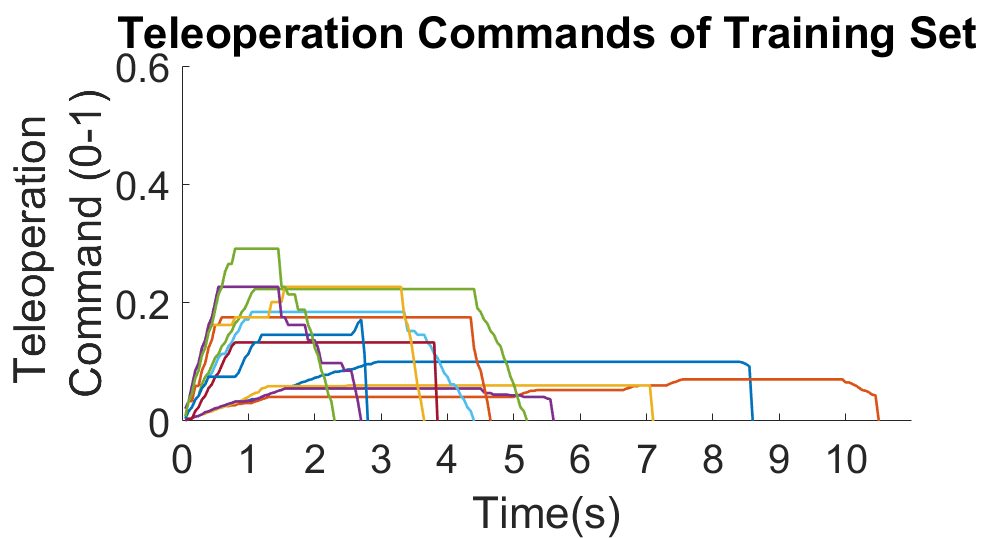
\includegraphics[width=0.49\linewidth]{images/traincommand.png}}
	\subfigure[Training Distances Travelled \label{fig:traintraj}]{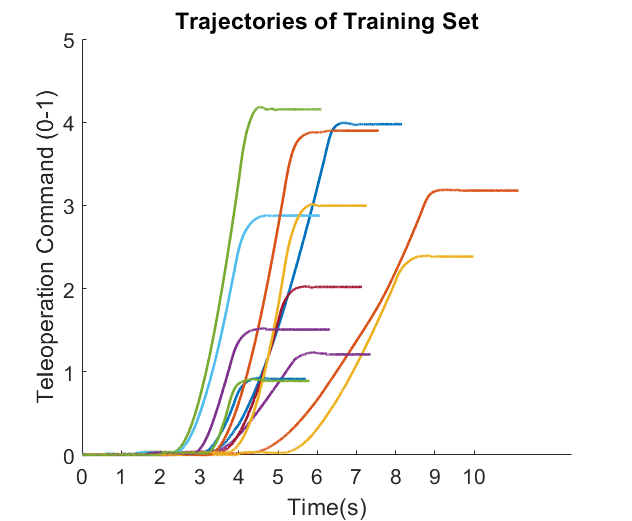
\includegraphics[width=0.49\linewidth]{images/trajset.png}}
	\caption{Training Set}
	\label{fig:train}
\end{figure}
%\NB{fix this figure axis...they are labeled wrong}\NB{Did you postprocess the axis and changed the values? The x axis is cut short..for example on the right the x axis should continue probably until 12 or 13...please use the matlab plot}\NB{change the title of the plots from Trajectories to Traveled Distances///trajectories are not only distances, they are a combination of dist, vel, acceleration etc}
%\NB{use subfigures and place the fig files for each figure in the repository so we can edit the figures. As we have discussed in the previous paper, titles and text in the figrue needs to be big and clear and readable and figrues need to span the entire column }
%\NB{rewrite stating that with these data we can train a model for trajectory starting and finishing with 0 speed. If the initial and final velocities are not 0...} 
With this data, we can train a model for trajectories that start and end with $0$ speed. This training would only be effective if trajectories involved stopping intermittently throughout the trajectory. Although in this work for ease of discussion, we focus on $0$ initial and final velocities, if a continuous motion throughout a trajectory is needed, then training can be executed on smooth trajectories by segmenting the existing training data to include trajectories for demonstrations where the velocity does not start and end at $0$ speed. Three separate types of segments will need to be evaluated in this case:
\begin{itemize}
    \item[a.] Start Trajectory, where the segment begins with a velocity of $0$ and ends with a given nonzero velocity $v$
    \item[b.] Intermediate Trajectory, where the segment begins and end with $v$ velocity
    \item[c.] End Trajectory, where the segment begins with $v$ velocity and ends with $0$ velocity
\end{itemize}
To expand the same data for this purpose, we train on portions of the training set pictured in Fig.~\ref{fig:train}, which correspond to each of the three outlined segments. The segments are formed by cutting the training data and trajectories at the start, the middle, and the end. Shown in Fig.~\ref{fig:trainelab} are four samples from our training set of the velocities and trajectories that correspond to the intermediary segments starting and finishing with the same velocity $v=0.4$m/s. %\NB{complete and fix the figure...the figure shows starting with 0.2 and ending with 0.4...Please cut the trajectories at 0.4 start and end}.
%ewe can extract the aformentioned segments from the training set - cut in a way that way obtain the desired initial and final conditions listed above.
\begin{figure}[H]
	\centering
	\subfigure[Training Intermediate Velocities \label{fig:trainvel}]{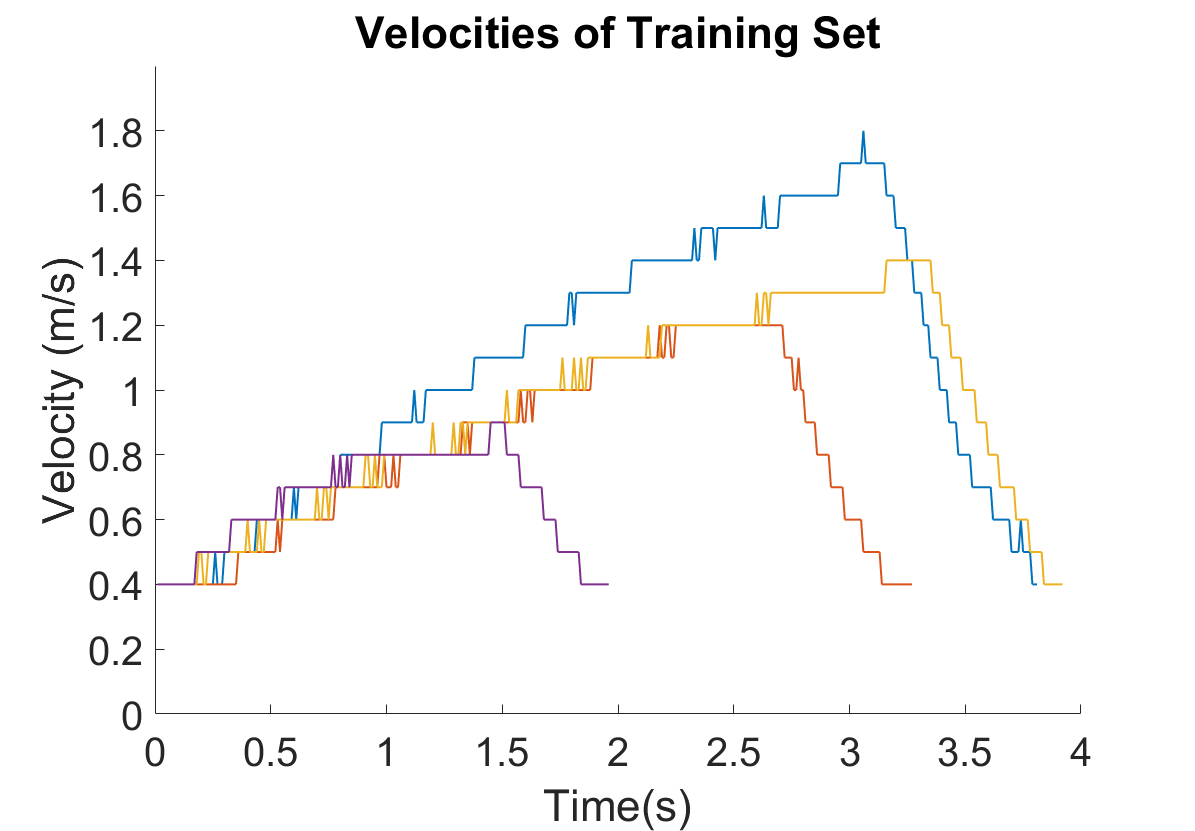
\includegraphics[width=0.49\linewidth]{images/trainelabvel.png}}
	\subfigure[Training Intermediate Trajectories \label{fig:trainteltraj}]{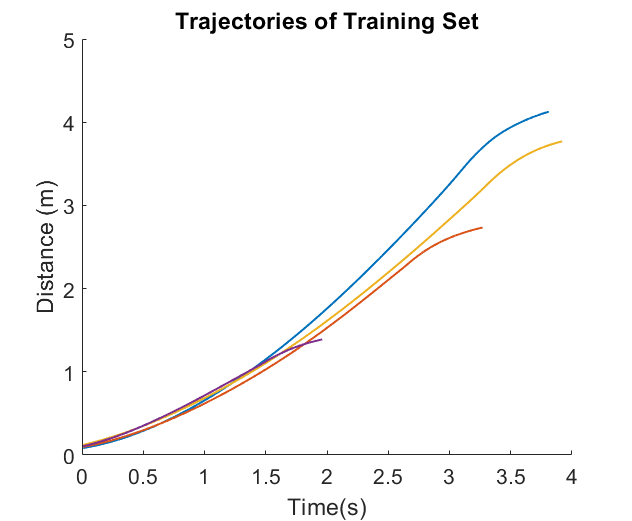
\includegraphics[width=0.49\linewidth]{images/trainelabtraj.png}}
	\caption{Intermediate Training Set}
	\label{fig:trainelab}
\end{figure}
%change pic to be accurate
%Training on not only trajectories that start and end with a velocity of $0$, but also on segments enables more specific command generation based on where the system is in relation to the provided trajectory. For example, if the command for the middle of the trajectory (i.e., between two points that are neither the start nor end of the trajectory) needs to be generated, then the training from the trajectories in Fig.~\ref{fig:trainelab} is used.

%\NB{you are not explaining well how you are doing this}
\subsubsection{Thin-Plate Spline Regression}

The offline training data is applied to a thin-plate spline (TPS) surface regression to describe the relationship between training inputs and integral and average input command. Given two inputs $x,y$, and the output $z$, the general form of a thin-plate spline equation is 
\begin{equation}
    f(x,y) = a_1 + a_xx + a_yy + \sum_{i=1}^mw_iU(||(x_i,y_i)-(x,y)||)
\end{equation}
%\NB{what you mean with average velocity?}
\NB{chnage x and y with new letters that you don't use in the paper for other variables.}
where $a_1,a_x,\text{and}~a_y$ are scalar coefficients, $w_i$ is a coefficient that corresponds to each data point, subject to the following smoothing condition: \begin{equation}
\sum_{i=1}^mw_i=\sum_{i=1}^mw_ix_i=\sum_{i=1}^mw_iy_i=0
\end{equation}
and the function $U$ is of the form
\begin{equation}
  U(r) = r^2\log{r} 
\end{equation}
where $r=||(x_i,y_i)-(x,y)||$.
Given the corresponding $z_i$ for each $(x_i,y_i)$ pair, we solve the following linear system to obtain the coefficients $w_i,\ldots,w_m$ and $a_1,a_x,a_y$,

\begin{equation}
    \begin{bmatrix}
    K&P\\
    P^T& \bm{0}
    \end{bmatrix}
    \begin{bmatrix}
    \bm{w}\\
    \bm{a}
    \end{bmatrix} = 
    \begin{bmatrix}
    \bm{z}\\
    \bm{o}
    \end{bmatrix}
\end{equation}

where $K_{ij} = U(||(x_i,y_i)-(x_j,y_j)||)$, each $i^{th}$ row of $P$ is $(1,x_i,y_i)$, $\bm{0}  \in \mathbb{R}^{3\times3}$ is a matrix of zeros, $\bm{o} \in \mathbb{R}^{3\times1}$ is a column vector of zeros, $\bm{w} \in \mathbb{R}^{m\times1}$ and $\bm{z} \in \mathbb{R}^{m\times1}$ are formed from $w_i$ and $z_i$, respectively, and $\bm{a}$ is the column vector with elements $a_1,a_x,a_y$.
%\NB{$P_i*$ does not appear in the equation}

Given the general framework for performing the thin-plate spline, we develop two separate relationships for our application. In our work, the first regression is applied to $d$ (distance traveled) and $t$ (time) as inputs to obtain the integral of the commands $g_i = f(d_i,t_i)$ while the second has the same inputs to obtain the average teleoperation command $\bar{j}_i = h(d_i,t_i)$. With the functions we have obtained, we are able to find an estimated integral and average input command, $g_u$ and $\bar{j}_u$, for any given desired distance and time, $d_u$ and $t_u$, respectively,
\begin{equation} \label{eq:integralfit}
g_u = f(d_u,t_u)
\end{equation}
\begin{equation} \label{eq:ssvelfit}
\bar{j}_u = h(d_u,t_u)
\end{equation}
In Figs.~\ref{fig:integs} and \ref{fig:joys}, we show the surfaces that represent the two functions $g_i = f(d_i,t_i)$ and $\bar{j}_i = h(d_i,t_i)$, respectively. The points in these figures represent actual training data points, all of which lay on the surface created with the thin-plate splines just introduced.

\begin{figure}[ht]
    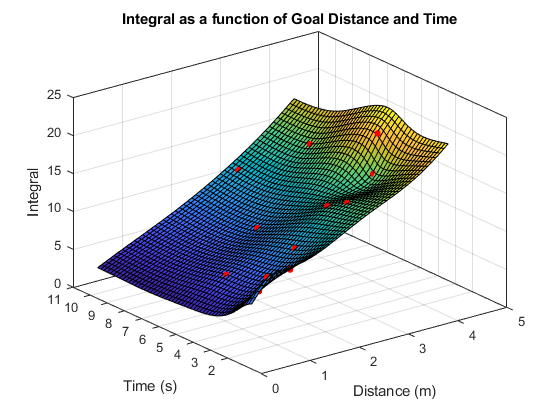
\includegraphics[width=0.48\textwidth]{images/integs.png}
    \caption{Integral vs Distance and Time}
    \label{fig:integs}
\end{figure}
\begin{figure}[ht]
    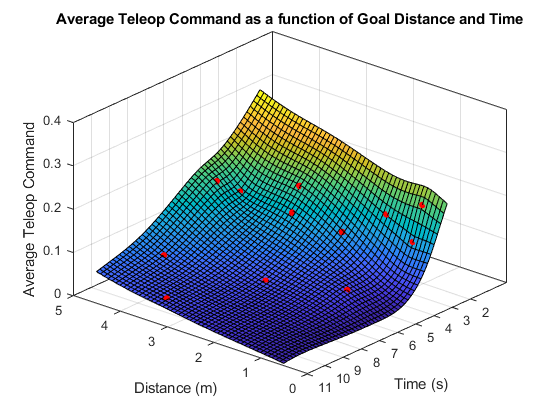
\includegraphics[width=0.48\textwidth]{images/joycmds.png}
    \caption{Average Teleoperation Input Command vs Distance and Time}
    \label{fig:joys}
\end{figure}
\subsubsection{Regression Error Analysis} \label{sec:regerror}
While a thin-plate spline is continuous, and a result can be obtained with any combination of distance and time as an input pair, the accuracy of the results of any pair $(d_u,t_u)$ can suffer as the distance between evaluation points and training points increases \cite{regress}. To deal with this problem, we consider the {\em standard error} of the estimate, which is a statistic that can be used to measure the accuracy of predictions given a certain type of regression \cite{stdereg} with known values, which are our training points:

\begin{equation} \label{eq:stderr}
    \sigma_{est} \approx \frac{s}{\sqrt{m}}
\end{equation}

where $s$ is the sample standard deviation of all of the points in the training set and $m$ is the number of training samples. The standard error, $\sigma_{est}$, is then used to determine the {\em t-statistic} for different test values \cite{tstat}. The t-statistic is defined as the ratio of the distance between a test point from a known training point to the standard error and is computed as follows:
\begin{equation} \label{eq:tstat}
t_{\hat{\beta}} = \frac{|\hat{\beta}-\bar{\beta}|}{\sigma_{est}}    
\end{equation}
where $\hat{\beta}$ is the test point and $\bar{\beta}$ is the nearest training point. In equation \eqref{eq:tstat}, $t_{\hat{\beta}} \geq 1$ indicates that the test point $\hat{\beta}$ propagates an error higher than the standard error. Therefore, it is desirable to have $t_{\hat{\beta}} < 1$. 
%\NB{what you mean with known? Do you mean training point?}
After selecting a desired set-point for the t-statistic, $t^*$, the maximum allowable departure from known points is $\sigma_{est}t^*$.

This maximum departure, $\sigma_{est}t_{\hat{\beta}}$, is used to set the bounds for each training data point, for example:
\begin{align}
    \beta_{\min} = \bar{\beta} - \sigma_{est}t^* \nonumber \\
    \beta_{\max} = \bar{\beta} + \sigma_{est}t^*
\end{align}
where $\beta_{\min}$ and $\beta_{\max}$ are the lower and upper bounds for any training point $\bar{\beta}$. %\NB{so each new testing point gets a different bound? Is it based only on the closest training point? What if we have 100 points close by? How do you take into account this situation that is different from having only 1 point} Adding a new test point changes the size of these ellipses because the std error changes.

In our case, there are two inputs we are primarily concerned about for prediction; distance and time, as in \eqref{eq:integralfit} and \eqref{eq:ssvelfit}. The distance and time values are used together as input pairs, so we use the convex hull around standard error ellipses to connect the two together \cite{stdellipse}. The standard error ellipse, in general, is computed as follows: %\NB{this section is too long..just go to the point. State that we are using this method to compute error region or whatever they are called} %\NB{I don't understand this..why are you separating this values? because we obtain a height and a length of these ellipses}
\begin{equation}
    \bigg(\frac{d}{\sigma_{d,est}t^*}\bigg)^2 + \bigg(\frac{t}{\sigma_{t,est}t^*}\bigg)^2 = 1
\end{equation}
where $d$ and $t$ represent values corresponding to the axes for distance and time, respectively, and $\sigma_{d,est}$ and $\sigma_{t,est}$, are standard error values for distance and time, representing the $x$ and $y$ axes of the TPS regression, respectively. The ellipses at each point in our training data are calculated using the following equations:
\begin{align} \label{eq:bounds}
    \bm{d}_i = d_i + \sigma_{d,est}t^*\cos{\theta} \nonumber \\
    \bm{t}_i = t_i + \sigma_{t,est}t^*\sin{\theta} 
\end{align}
where $\theta$ is an angle from $[0,\ldots,2\pi]$, and $\bm{d}_i$ and $\bm{t}_i$ are all of the points on the perimeter of the ellipse for training point $(d_i,t_i)$, and $i = 1,\ldots,m$ where $m$ reflects the total number of training points. A convex hull is then computed around the ellipses to provide a concise measure for the combination of distances and times that result in low error outputs when input into the TPS regression. This convex hull is generated using the Quickhull algorithm \cite{quickhull}, in which we take the outermost points of the set ellipses and form a boundary denoted $Conv(M)$, where $M$ represents the set of all points on the perimeters of all ellipses: $\{\bm{d}_i,\ldots,\bm{d}_m\},\{\bm{t}_i,\ldots,\bm{t}_m\}$.

In Fig.~\ref{fig:preds}, the convex hull around standard error ellipses created with $t^* = 0.5$ around each training point is depicted. Fig.~\ref{fig:predsur} is the TPS regression model for the integral \eqref{eq:integralfit} overlaid with the convex hull \cite{bounds} created from the ellipses on Fig.~\ref{fig:preds}.
\begin{figure}[H]
	\centering
	\subfigure[Prediction Bounds \label{fig:preds}]{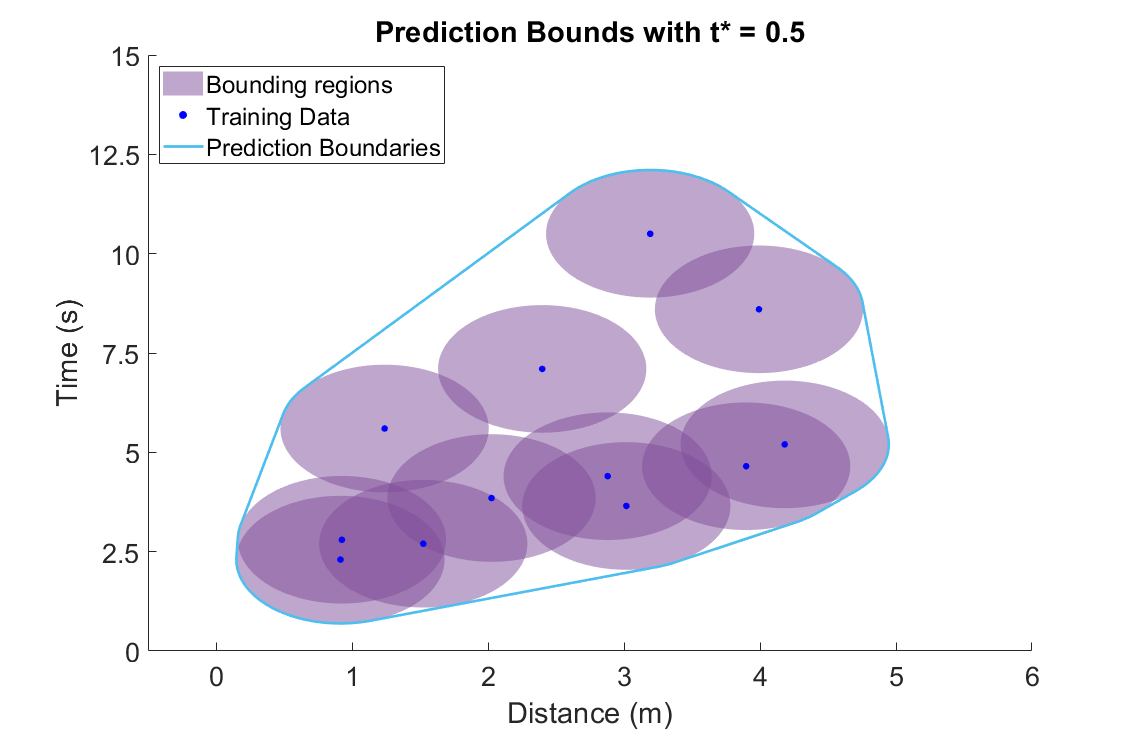
\includegraphics[width=0.49\linewidth]{images/predictionbds.png}}
	\subfigure[Prediction Bounds on Surface \label{fig:predsur}]{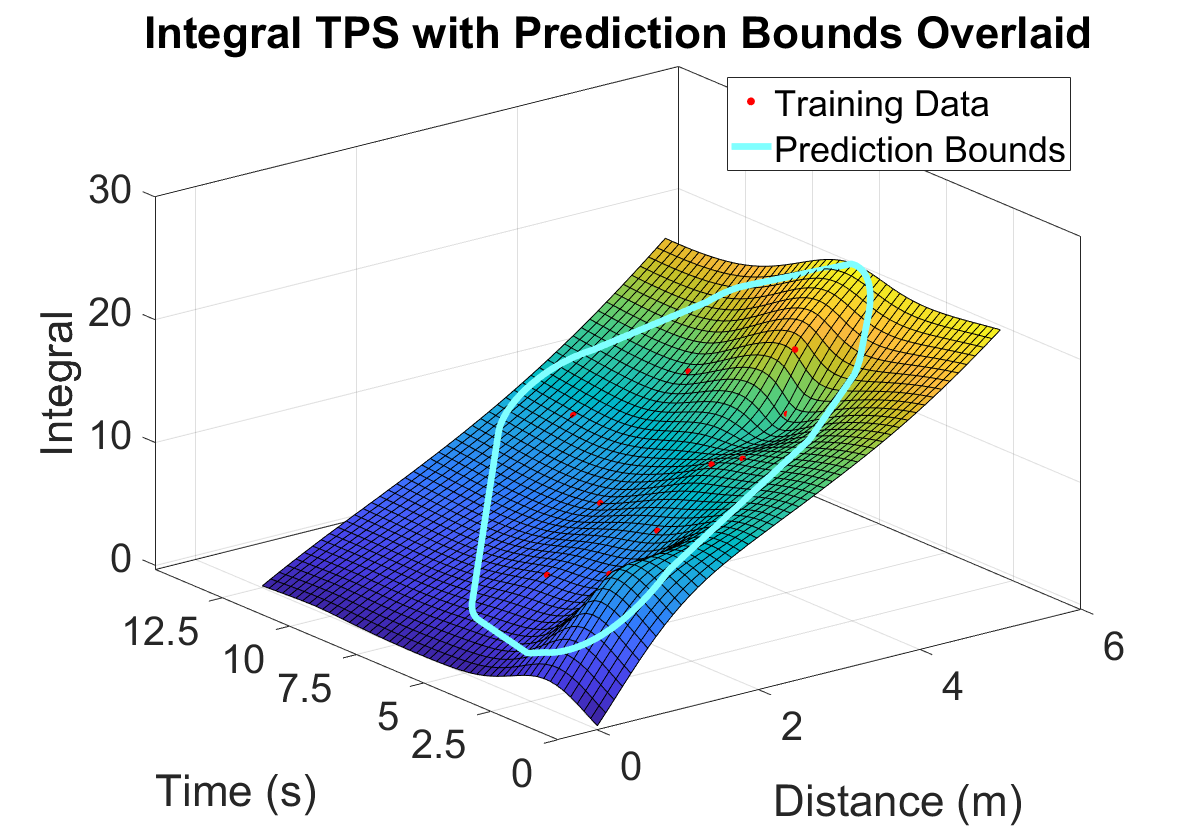
\includegraphics[width=0.49\linewidth]{images/fulpredbds.png}}
	\caption{Prediction Intervals and Bounds}
	\label{fig:bounds}
\end{figure}
An alternate method would have been to use standard error rectangles\cite{stdellipse} instead, which create rectangular intervals around each data point, but these are not necessarily accurate for smoothed surfaces, as rectangular regions would have non-differentiable corners, which are incongruous with smoothing conditions met by the TPS regression. 

With this analysis, we are able to provide boundary conditions for our training set, when determining what kind of trajectories we can follow. In the next section, we discuss how we build trajectories and how we use these boundaries with a satisfiability modulo theories (SMT) solver \cite{smt} to ensure that our UAV can indeed track generated trajectories.
%\NB{so what's the punchline here? We need to say what you obtain with this analysis and perhaps connect with the SMT Solver later}
%The prediction bounds presented here satisfy the smoothness condition of our regression and are used to generate trajectories, which is discussed in the next section. 
%\NB{we need to state what we do if they are not good}\NB{you mention this later. You need to anticipate the reviewer reaction. Here you need to mention that in the next section we show what to do if the result of this test is negative or you need to present here directly}

\subsection{Trajectory Generation and Decomposition} \label{sec:traj}
In this section, we discuss how we generate, discretize, and decompose smooth trajectories, subject to the regression error analysis presented in the previous section.
%, which is verified with an SMT solver.
Relating back to the system dynamics, we have established that input commands are responsible for specific motions of the system. Roll enables lateral motion while pitch enables longitudinal motion. Therefore, any planar motion assuming constant $z$ and $\psi$ can be represented as a combination of roll and pitch commands, or commands that move the vehicle along the global $x$ and $y$ coordinates. Hence when considering a planar $x,y$ trajectory we perform a decomposition in the $x$ and $y$ directions and generate independent roll and pitch commands to follow simultaneously trajectories in the $x$ and $y$ directions, respectively. 
%each trajectory simultaneously.
%Because the using just roll and pitch commands is possible, we desire to decompose the trajectory into $x$ and $y$ components, as any smooth trajectory can be represented as a combination of these components.
%\NB{this section needs to go before and needs to be explain better}.
In order to generate a trajectory, we first select waypoints through which the UAV should travel. The optimal path is then determined by using a minimum snap trajectory. Minimum snap trajectories are associated with low control effort as they are based on the fourth derivative of position and ensure smoothness on quadrotors which have been proven to be 4th order systems \cite{minsnap}. The general equation for a minimum snap trajectory is the solution of the following functional:
%\NB{why? you need to explain better. Besides, we should use snap not jerk}
\begin{equation} \label{eq:minjerkint}
%    \bm{p}^*(t) = \argmin_{p(t)}\int_0^T\mathcal{L}(\ddddot{p},\dddot{p},\ddot{p},\dot{p},p,t)dt
    \bm{p}^*(t) = \argmin_{p(t)}\int_0^T(\ddddot{p})^2dt
\end{equation}
%\NB{I've correct the expression above}
%Solving \eqref{eq:minjerkint}, we obtain the form:
%\begin{equation}
%    \bm{p}^*(t) = c_7t^7 + c_6t^6 + c_5t^5 + c_4t^4 + c_3t^3 + c_2t^2 + c_1t + c_0 
%\end{equation}
%where $c_0,\ldots,c_7$ are constants associated with specific waypoints in the trajectory.%\NB{this is incorrect. Are you doing this in your simulation???}
\NB{we need to think if these equations are really necessary here. for now leave them but keep the comment}
The obtained smooth trajectory is then discretized into $n$ segments.

Each segment will have a time-step of $\Delta t = \frac{T}{n}$, where $T$ is the total amount of time allotted for the full trajectory. The discretization is done using linear interpolation within the trajectory over each interval $[\bm{p}^*(t_i), \bm{p}^*(t_i+\Delta t)]$, where $t_i$ is the time at the start of a segment $i=1, \ldots, n-1$. Here $t_1=0$ and $t_n=T$. 
% and $t_{s+1}$ is the end of the segment, defined as: $t_{s+1} = t_s + \Delta t$. 
%\NB{why so complicated this description...please simplify you are just doing a discretization. Also correct gramamr }.
%\NB{please write the mathematical expression for the x and y component from the trajectory otherwise this section is incomplete}
%\NB{several? they are just 3...please ad the decomposition otherwise this section is useless}
Some examples of discretized trajectories are shown in Fig.~\ref{fig:trajs}. 
\begin{figure}[h]
	\centering
	\subfigure[\label{fig:t1}]{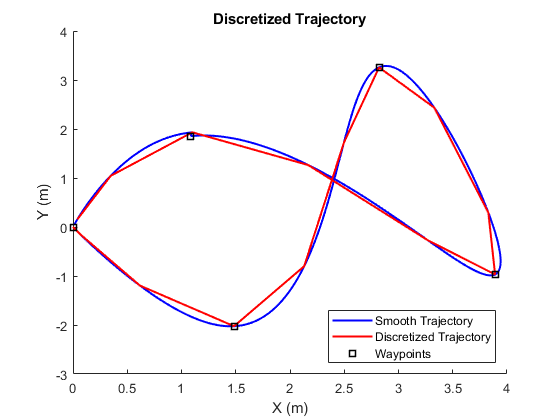
\includegraphics[width=0.3\linewidth]{images/traj1.png}}
	\subfigure[\label{fig:t2}]{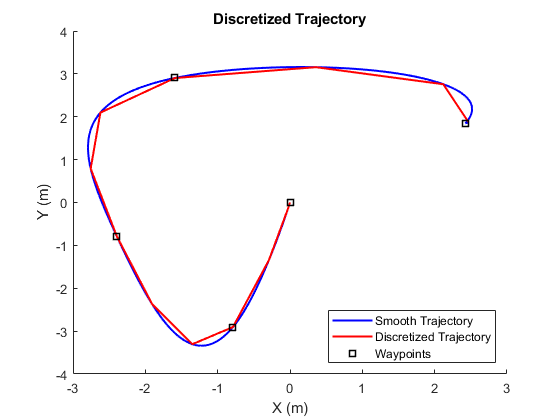
\includegraphics[width=0.3\linewidth]{images/traj2.png}}
    \subfigure[\label{fig:t3}]{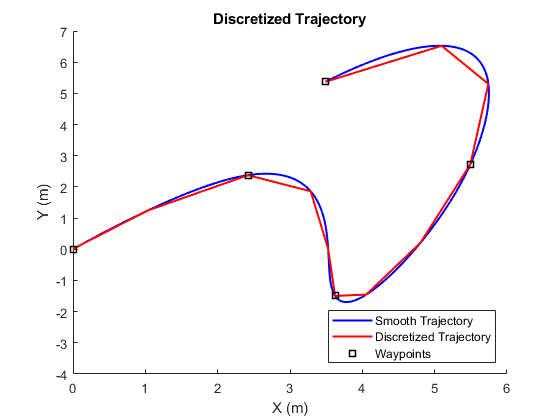
\includegraphics[width=0.3\linewidth]{images/traj3.png}}
	\caption{Examples of discretized trajectories. All of the trajectories start at the world frame origin $(0,0)$.}
	\label{fig:trajs}
\end{figure}

From the discretized trajectory, we can obtain the $x$ and $y$ components of each leg of the trajectory. All components can then be composed in a sequence obtaining two trajectories in the $x$ and $y$ directions as follows:
\begin{align}
    \bm{p}_x^*&=\left[ \bm{p}_x^*(t_1), \bm{p}_x^*(t_2), \ldots, \bm{p}_x^*(t_{n})\right] \nonumber \\
    \bm{p}_y^*&=\left[ \bm{p}_y^*(t_1), \bm{p}_y^*(t_2), \ldots, \bm{p}_y^*(t_{n})\right]
\end{align}

Fig.~\ref{fig:t2dec} shows an example of a generated trajectory with its discretization while Fig.~\ref{fig:tdec} displays the $x$ and $y$ sequences together.
\begin{figure}[ht]
	\centering
	\subfigure[Discretized Trajectory\label{fig:t2dec}]{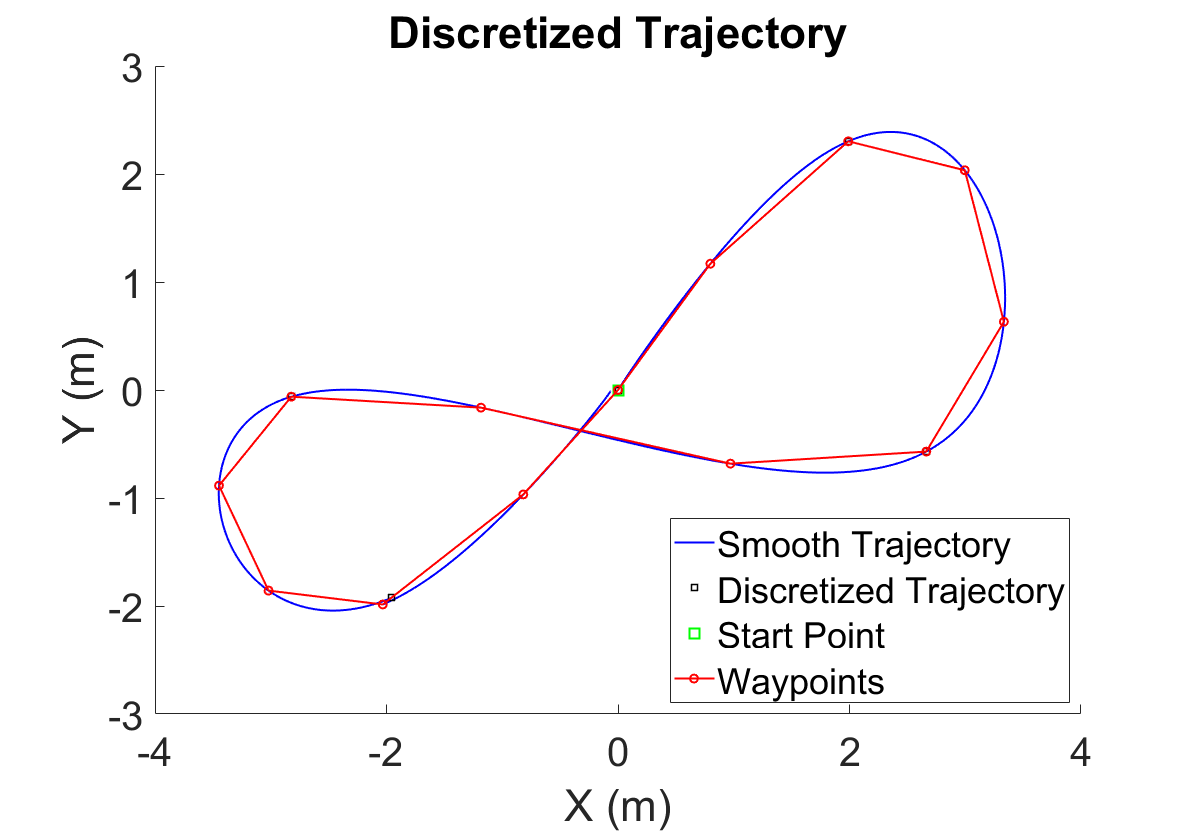
\includegraphics[width=0.48\linewidth]{images/traj2dec.png}}
	\subfigure[X and Y Components\label{fig:tdec}]{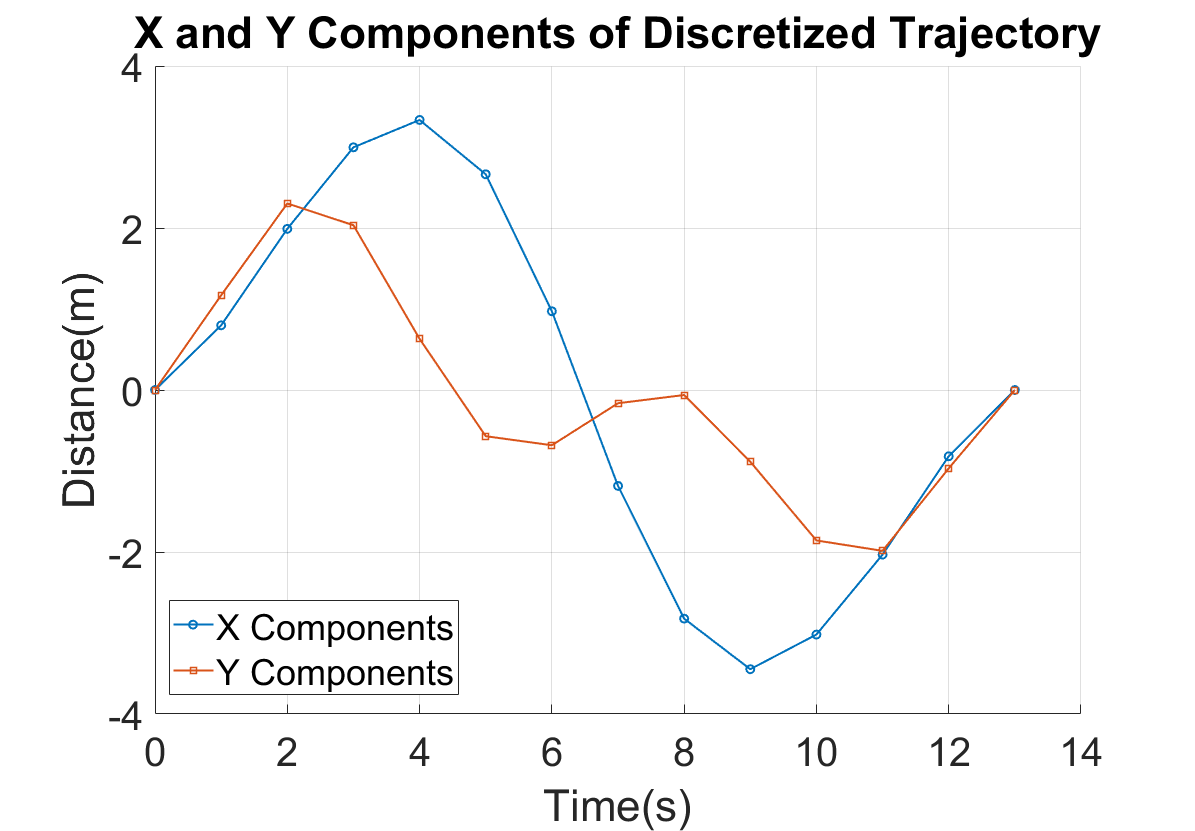
\includegraphics[width=0.48\linewidth]{images/trajdecomp.png}}
	\caption{Example of a Generated Trajectory with its $x,y$ Decomposition}
	\label{fig:trajdec}
\end{figure}

%In Fig.~\ref{fig:tdec}, we show the components at each interval. 
These components, when executed simultaneously, correspond to the discretized trajectory pictured in Fig.~\ref{fig:t2dec}. The smaller $\Delta t$ is, better is the approximation of the smooth trajectory. Each of the components are then evaluated with the prediction bounds from Fig.~\ref{fig:bounds}. If the error regions are violated, there is a possibility that the UAV will not reach the points in the discretized trajectory. To resolve this issue, we use an SMT solver, which is a verification tool that solves a first order satisfiability problem. In our work, the condition that we want to satisfy is that each of the distances and their corresponding time is within the convex hull, $Conv(M)$ presented in Section~\ref{sec:regerror}. Using an SMT solver, we check if all the distances in both components $\bm{d}_{x,i}=||\bm{p}_x^*(t_i+1)-\bm{p}_x^*(t_i)||$ and $\bm{d}_{y,i}=||\bm{p}_y^*(t_i+1)-\bm{p}_y^*(t_i)||$ are attainable in time-step $\Delta t$ subject to $Conv(M)$ : 
\begin{equation}\label{eq:smt}
%    (\bm{p}_x^*(t_i),\Delta t) \wedge (\bm{p}_y^*(t_i),\Delta t) \in Conv(M)
    (\bm{d}_{x,i},\Delta t) \wedge (\bm{d}_{y,i},\Delta t) \in Conv(M), ~\textrm{with}\, i = 1,\ldots,n-1
\end{equation}
%where $i = 1,\ldots,n-1$. 
If this condition is satisfied, then the trajectory is feasible. If not, and if there exists a solution, the solver returns a time-step $\Delta t^*$ for each segment of the trajectory that satisfies the condition in \eqref{eq:smt} together with the following constraint
\begin{align}
%     (\bm{p}_x^*(t_i),(t_{i+1}-t_i)) &\wedge (\bm{p}_y^*(t_i),(t_{i+1}-t_i)) \in Conv(M) \nonumber \\
     \sum_{i=1}^n(t_{i+1}-t_i) = T
\end{align}
to ensure that the sum of the new time-steps is the total time allotted for the trajectory $T$, while also ensuring that any segment has a distance-time pair within the convex hull $Conv(M)$. If the solver still cannot obtain a result, it is indicative of an unattainable distance or distances within the trajectory, indicating that the trajectory as a whole is unattainable, and the waypoints need to be changed for example by increasing $n$ and reducing $\Delta t$. Provided that all of the conditions for the SMT solver are met, we can obtain the correct $x$ and $y$ trajectory components and their corresponding times. We now discuss the command generation procedures that we use to enable autonomous tracking of trajectories.
%\NB{it may be better to show the trajectory generation later}



\subsection{Autonomous Input Generation} \label{sec:generate}

In order for the system to autonomously reach a waypoint generated by the discretized trajectory, %\NB{what does it mean to reach a point within trajectory. This is super confusing.Are you trying to reach a point within the trajectory? I thought we are trying to track a trajectory from the beginning to the end(?) This is what a reviewer will ask here. Please be more precise and refer to the waypoint generated by discretizing the trajectory}
$g_u$ and $\bar{j}_u$ are obtained using equations \eqref{eq:integralfit} and \eqref{eq:ssvelfit} with each component of our trajectory, and the offline training samples are leveraged to generate a new string of commands. From the training set of $m$ samples, we select the trial that has the closest integral, $g_i$, to the estimated integral $g_u$. This is done by forming an error vector, $\bm{e}\in\R^{m}$, where each element is defined by
\begin{equation}
 e_i = \vert g_i-g_u \vert , ~i= 1,\ldots,m
\end{equation}
 The lowest error in $\bm{e} = \{e_1,\ldots,e_m\}$ is then found and paired with the appropriate pre-trained sample, $\bm{J}^*$, %\NB{show $\bm{e}$}
\begin{equation}
\bm{J}^* = \bm{J}_i \in \bm{J}\vert e_i = \min_e(\bm{e})
\end{equation}

This closest pre-trained sample is then adjusted to reflect the user-set time, $t_u$ by performing bicubic interpolation, so that important features in the optimal command vector are not lost. Interpolation methods are often used for re-sizing complex images, and have shown effectiveness in minimizing feature loss \cite{bicfeatures}. Bicubic interpolation is the chosen method for re-sizing, as it performs better than nearest-neighbor and bilinear interpolation methods, while only marginally increasing computational complexity \cite{biccomp}. The general form of a bicubic interpolation equation is: 
%\NB{there are too many ``This is done" in this section. They brake the flow of the paper...go to the point ...This optimal pre-trained sample is then adjusted to reflect the user-set time, $t_u$ by performing...}

\begin{equation} \label{eq:bicinter}
    b(x) = \sum_{i=0}^3c_ij^i
\end{equation}

where $j$ is an entry in vector $\bm{J}^*$ and $c_i$ represents the coefficients of the best-fit cubic function at each point. %\NB{no clue what this means...what are these coefficients? coefficients of the cubic best fit to find the values that would go in between each entry}.
Bicubic interpolation takes the weighted sum of the four nearest neighbors of each entry in the command vector in order to identify a function for the intermediate points around each entry in $\bm{J}^*$. This method is a result from \cite{bicfeatures}, where it is described in more detail. After resizing, the time adjusted input vector $\bm{J}'$ is obtained.

The next step is to adjust the input vector such that the system reaches the waypoint at distance $d_u$ by leveraging the average input command information $\bar{j}_u$. Because we have identified in Section~\ref{sec:sysdyn} that distance is a function of this average input command and time, the time-adjusted vector $\bm{J}'$ is scaled such that its mean is equivalent to $\bar{j}_u$:
\begin{equation} \label{eq:imgscale}
\bm{J}'' = \bm{J}'\bigg(\frac{\bar{j}_u}{\bar{j}'}\bigg)
\end{equation}
Lastly, we correct for integral error. While using the fitted average input, $\bar{j}_u$, scales the commands, there may still be some error between the integral of our new command string and the desired integral, $g_u$. The ratio between the two integrals is leveraged to re-scale the command string:
\begin{equation} \label{eq:iintscale}
\bm{J}_a = \bm{J}'\bigg(\frac{g_u}{\int_0^{t_u}\bm{J}''dt}\bigg)
\end{equation}


In Fig.~\ref{fig:gensample}, each step of the command generation process is visualized, starting with the original pre-trained command string in Fig.~\ref{fig:ogstring}. This flight lasted approximately $4.4$ seconds for $3$ meters. For testing purposes, the user input values are $d_u=3.5$m and $t_u=3.75$s. As indicated, a time adjustment is made first; this is shown in Fig.~\ref{fig:timeadj}. It is important to note that the average command, indicated by the dashed line, is still the same, which is a verification of feature retention aspect of bicubic interpolation from \eqref{eq:bicinter}. If the command string were adjusted without using an interpolation method, there may be slight variation in the mean, which could damage the integrity of the final command string, shown in Fig.~\ref{fig:fullyadj}, which is obtained using \eqref{eq:imgscale} and \eqref{eq:iintscale}. At this point we have obtained the autonomous command string $\bm{J}_a$, which is then sent to the UAV to reach a waypoint within the generated trajectory.

\begin{figure}[h]
	\centering
	\subfigure[Original String \label{fig:ogstring}]{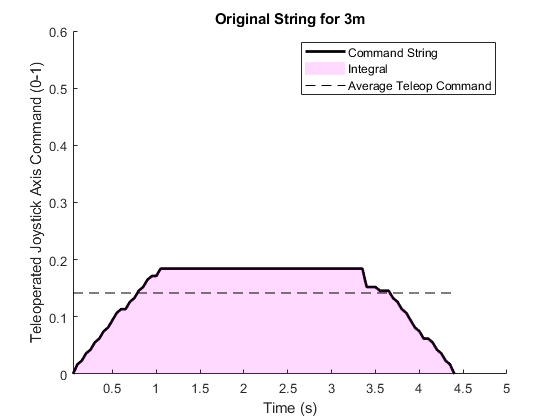
\includegraphics[width=0.3\linewidth]{images/ogstring.png}}
	\subfigure[Time Adjustment \label{fig:timeadj}]{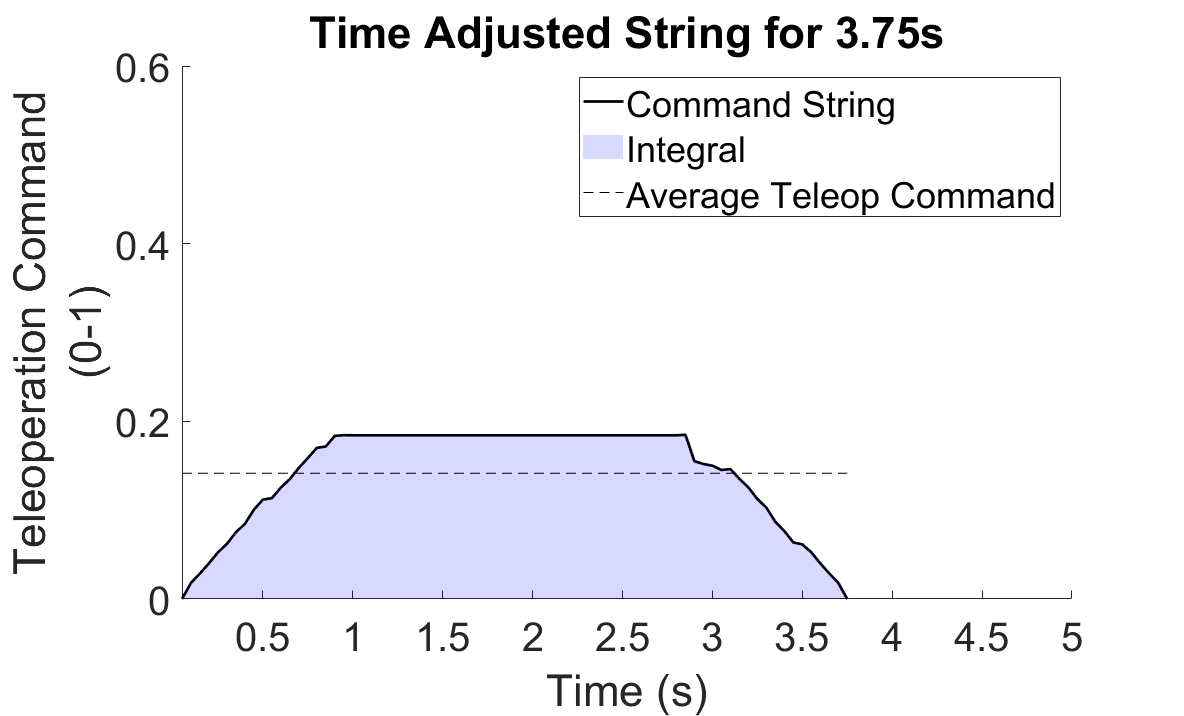
\includegraphics[width=0.3\linewidth]{images/timeadj.png}}
    \subfigure[Final Commands \label{fig:fullyadj}]{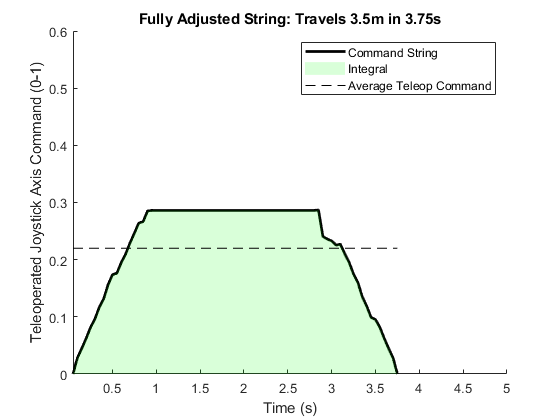
\includegraphics[width=0.3\linewidth]{images/fullyadj.png}}
	\caption{Command Generation Process}
	\label{fig:gensample}
\end{figure}

From the autonomous command, the expected path of the vehicle is generated. The integral of the final command string is taken at each time-step to determine the expected position at all times:
\begin{equation}
    g_J(t) = \int_0^t\bm{J}_a dt
\end{equation}
Because we know the relationship between the integral and the distance travelled at all times, we are able to leverage the equation from the TPS regression for the integral, \eqref{eq:integralfit}, such that the inputs are time elapsed and integral of the autonomous command string and the output is the distance traveled: %\NB{this sentence doesn't make sense}:
\begin{equation} \label{eq:distresult}
d_J(t) = f^{-1}(g_J(t),t)
\end{equation}
where $g_J(t)$ is the integral of the string of generated commands at time $t$, and $d_J(t)$ is the resultant distance travelled at $t$.

%\NB{where is the part of the text in which you show how to generate the prediction of the position occupied by the vehicle by following the determined sequence of inputs?}
\subsection{Online Adaptation of Generated Commands} \label{sec:adapt}

The commands generated in the previous section are generated and sent to the UAV in open-loop. While the open-loop autonomous controls generated in this manner may be reasonably accurate, we desire more assured trajectory tracking by controlling for any possible error, thereby closing the loop. While executing the generated command string, $\bm{J_a}(t)$, we monitor the error between the position of the vehicle, $\bm{p}(t)$ and the reference position as per the generated trajectory, $\bm{p_r}(t)$:
\begin{equation}
    \xi(t) = \bm{p_r}(t)-\bm{p}(t)
\end{equation}
%\NB{is $\xi$ a vector?}

This error at time $t$, $\xi(t)$, is attributed to the most recent command sent to the system. A proportional controller is implemented to adjust the subsequent command, $\bm{J}_a(t+1)$, to obtain the closed-loop command $\bm{J}_c(t+1)$ as follows:
\begin{equation}
    \bm{J}_c(t+1) = \bm{J}_a(t+1) + k_p\xi(t)
\end{equation}
%\NB{mention why you are doing this that is because in this way the corrective action is not too high and tailored based on the command that on average it should receive and thus do not overshoot}
In our work, the controller gain, $k_p$, is a static value that is set based on the input being provided to the system as follows:
\begin{equation} \label{eq:ctrls}
    k_p = r_p\bar{j}_a
\end{equation}
where $\bar{j}_a$ is the average input from the open loop commands and $r_p$ is a ratio applied to the average input. The gain is chosen in this manner as to avoid drastic corrections that would affect the stability of the system. If the error at time $t$, $\xi(t)$, is very high, then having $r_p \geq 1$ could result in a drastic and unstable change in the control input. The set value of the correction ratio depends on the amount of adjustment desired by the user, which depends on certain constraints, such as flight time and flight conditions, i.e., different correction ratios may be desirable for indoor and outdoor flight. Using this controller, the position error is lowered to ensure that the UAV does indeed reach the generated waypoint as expected.  %\NB{what threshold?} 

%where $t_u$ refers to the user-set time, and adjusts the update of $k_p$ such that the rate of increase is controlled for iteration time. If the rate of increase is not controlled in this manner, it would suggest that the controller is controlling for error over the entire remaining string of commands, rather than the first subsequent command. Each subsequent command is adjusted because our positional liveness constraint is defined as maintaining a certain distance between actual and reference positions at all times, from \eqref{eq:positlive}. If the constraint was for the UAV to reach the goal at a certain time immaterial of the path/trajectory, adjusting the entire remaining portion of the command string would be ideal.


\section{Experiments} \label{sec:exper}
%\NB{we need the overlapped sequence of pictures for the different experiments besides the UVA one. }
The proposed approach was validated experimentally using a Parrot BeBop 2 quadrotor UAV, which is tuned and stable for teleoperation off-the-shelf. Since experiments were conducted indoors, a Vicon motion capture system was used to obtain the position and velocity of the vehicle. Alternatively, one could use GPS and IMU data to obtain similar features in different conditions. 
%The teleoperation was performed using a node written in the ROS environment.

The training set was generated by having a human teleoperate the system $12$ times with motion that only consisted of forward pitch commands. The user was instructed to fly different distances with different speeds to diversify the training set. We also used this same training set to generate roll commands for our UAV since the vehicle is symmetric.

The regression and error analysis was done in Matlab to obtain the surfaces pictured in Section \ref{sec:train}, and are shown in Figs.~\ref{fig:integs}, \ref{fig:joys}, and \ref{fig:bounds}. The experiments were conducted using ROS in conjunction with the Robotics System Toolbox in Matlab to interface our regression models and generated commands with the UAV.

The first experiments consisted of tracking a diagonal distance, to validate that $x$ and $y$ components as discussed in Section~\ref{sec:traj} can be attained accurately. Starting from the world frame origin, we set the target to $(-1.7,2.3)$, that is, $-1.7$m in the $x$ direction and $2.3$m in the $y$ direction. The time set for this trajectory was $5.25$s. Using the regression training, we obtain the open-loop commands for the $x$ and $y$ directions, which are pictured in red in Figs.~\ref{fig:xcmds} and \ref{figs:ycmds}, respectively. The open-loop commands yield the trajectory in Fig.~\ref{fig:1723open}.

To show the effect of our adaptive controller, we ran the same experiment with our controller, and compared results obtained in open and closed loop systems. In Fig.~\ref{fig:1723controlled}, the real-time adapted inputs and the error associated with each of the trials in the $x$ and $y$ directions are shown. In Fig.~\ref{fig:x2traj}, we show the distance traveled in $x$ with the commands pictured in blue from Fig.~\ref{fig:xcmds}, which are generated due to the error indicated in Fig.~\ref{fig:xerr}. The blue line in this figure indicates the error converges to $0$. In Figs.~\ref{fig:yerr},~\ref{fig:ycmds},~\ref{fig:y2traj}, the same results are shown for movement in the $y$ direction.

\begin{figure}[ht]
	\centering
	\subfigure[X Error \label{fig:xerr}]{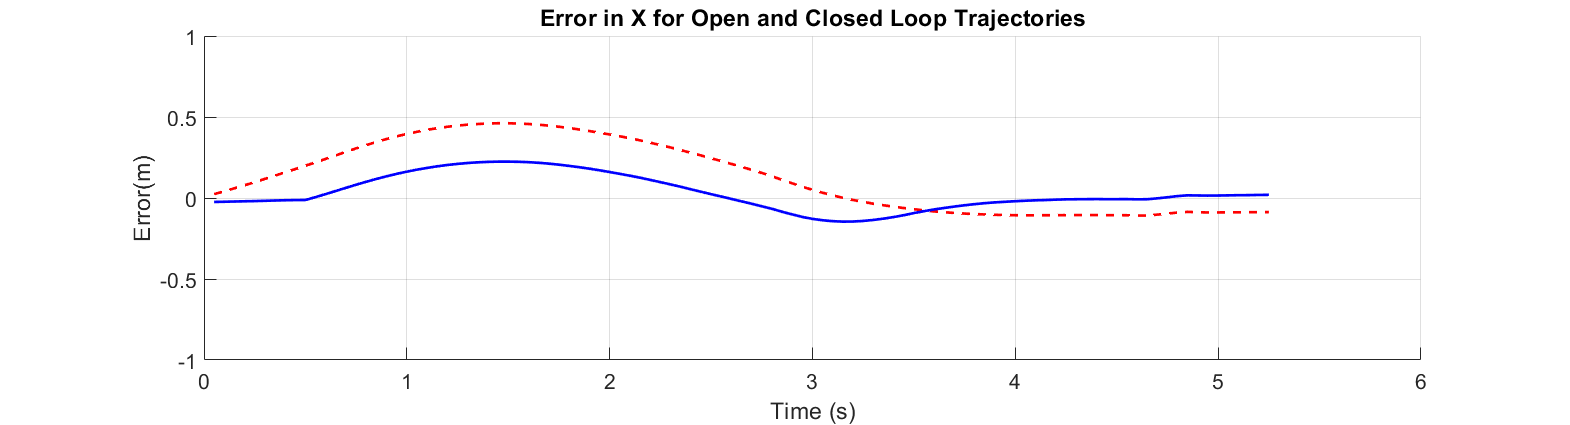
\includegraphics[width=0.9\linewidth]{images/XERR.png}}
    \subfigure[X Commands \label{fig:xcmds}]{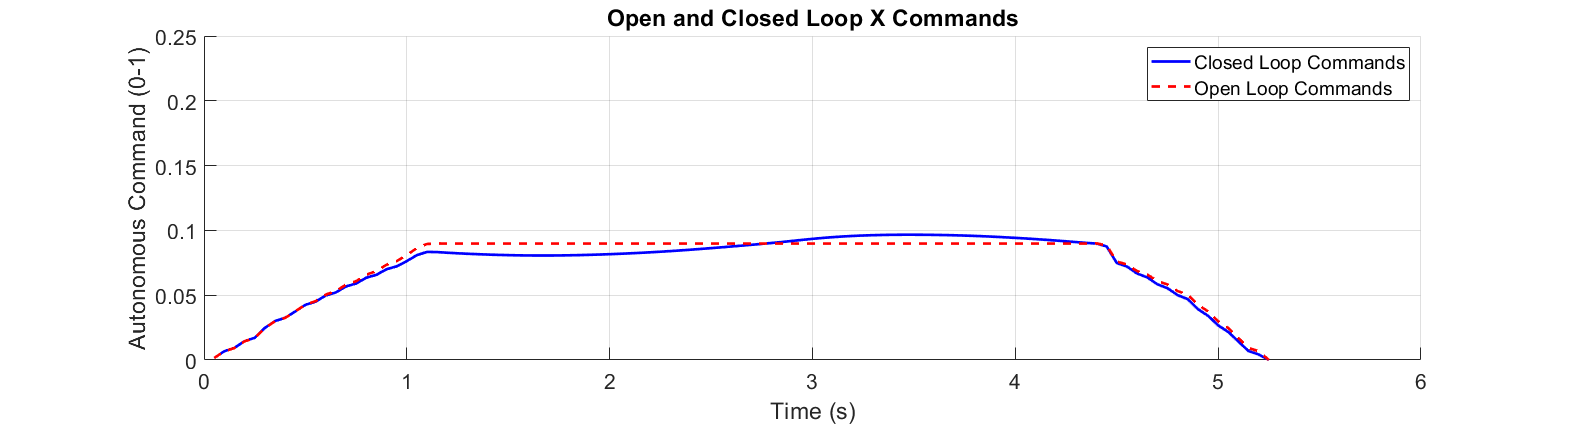
\includegraphics[width=0.9\linewidth]{images/CLOSEDXcmds.png}}
    \subfigure[X Distance Traveled in Open and Closed Loop \label{fig:x2traj}]{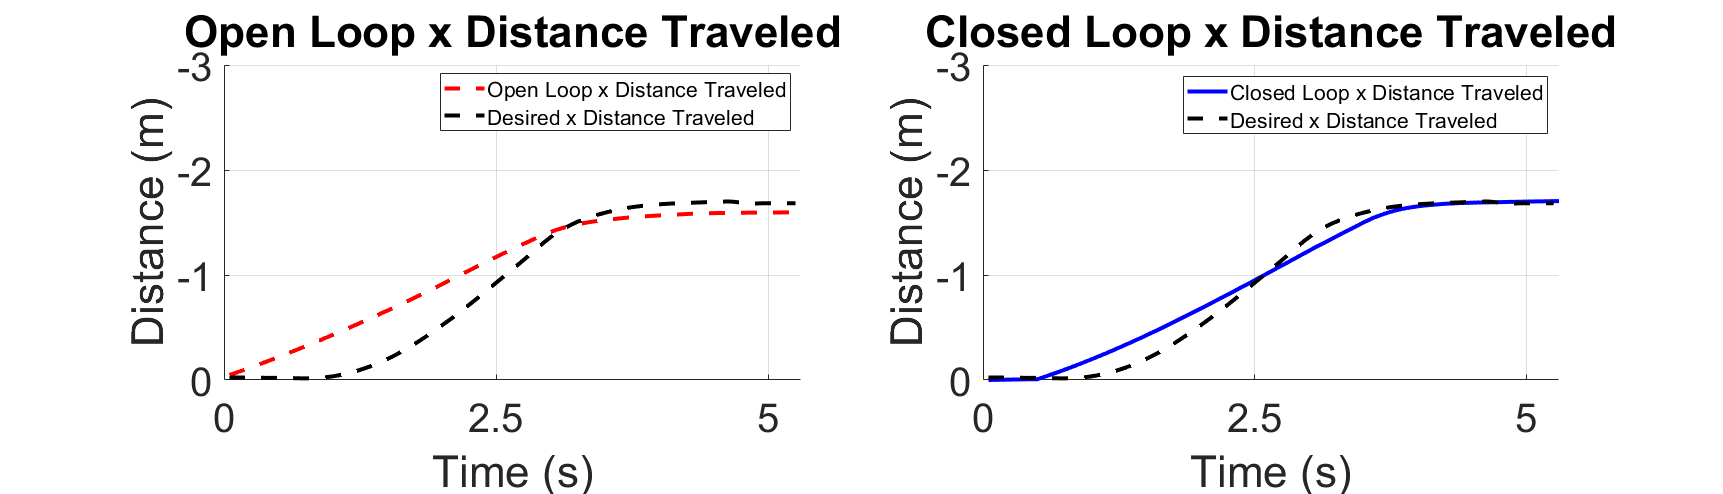
\includegraphics[width=0.9\linewidth]{images/Xtrajs.png}}
    \subfigure[Y Error \label{fig:yerr}]{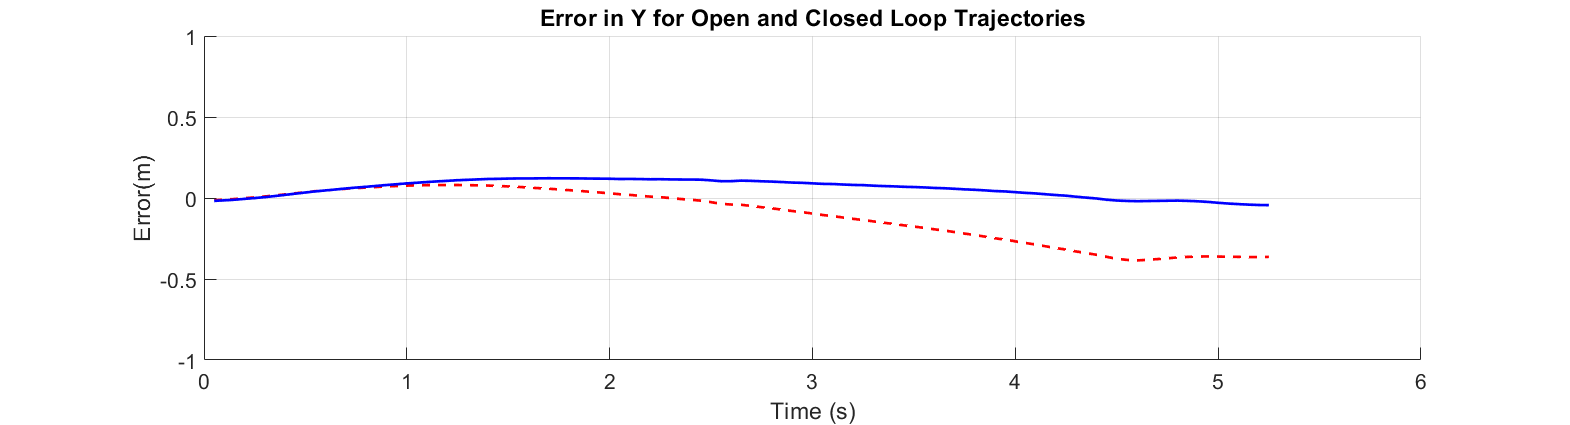
\includegraphics[width=0.9\linewidth]{images/YERROR.png}}
    \subfigure[Y Commands \label{fig:ycmds}]{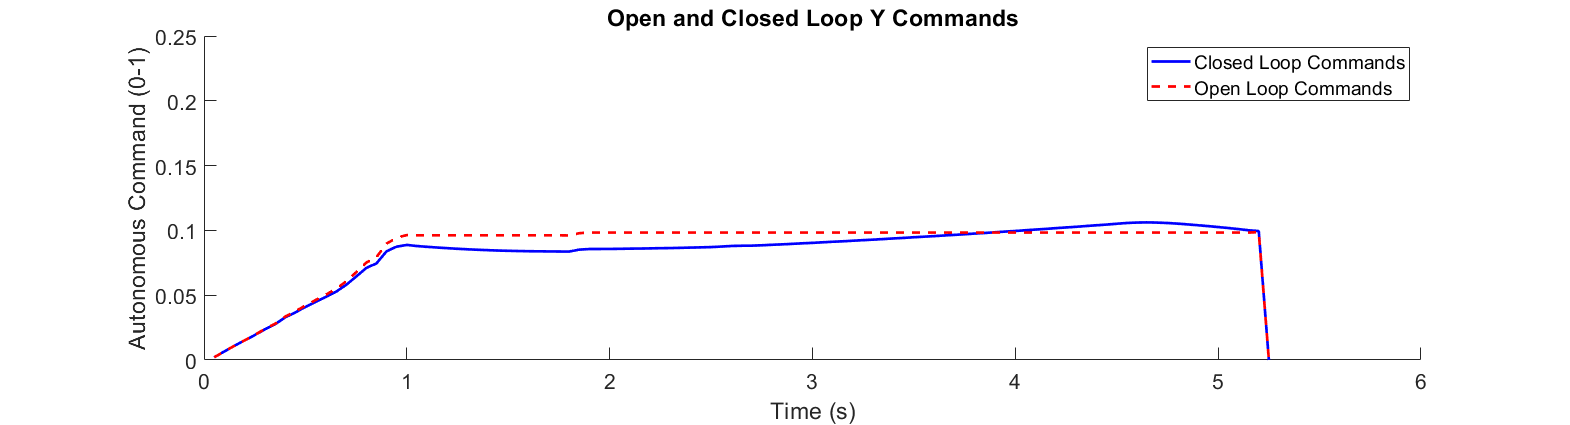
\includegraphics[width=0.9\linewidth]{images/CLOSEDYcmds.png}}
    \subfigure[Y Distance Traveled in Open and Closed Loop \label{fig:y2traj}]{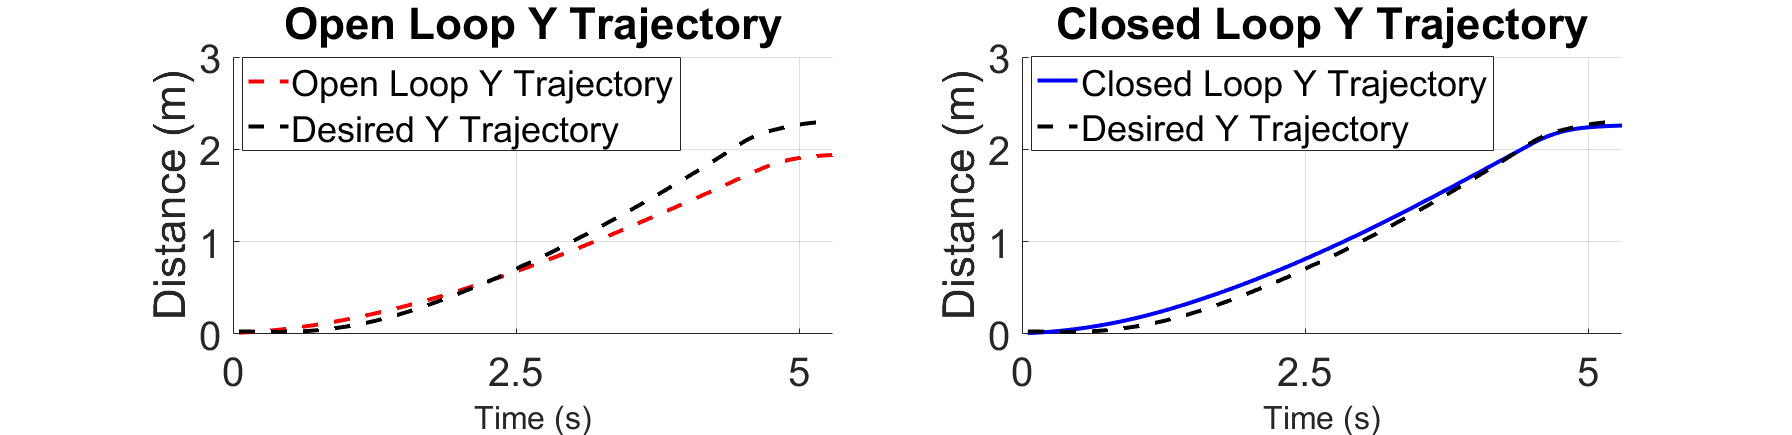
\includegraphics[width=0.9\linewidth]{images/Ytrajs.png}}
	\caption{Error and Control in the X and Y Directions}
	\label{fig:1723controlled}
\end{figure}

The resultant diagonal trajectory is shown in Fig.~\ref{fig:1723trajs}, and \ref{fig:diagquad} is an image of the experiment.
\begin{figure}[ht]
    \centering
	\subfigure[Open Loop Diagonal Experiment\label{fig:1723open}]{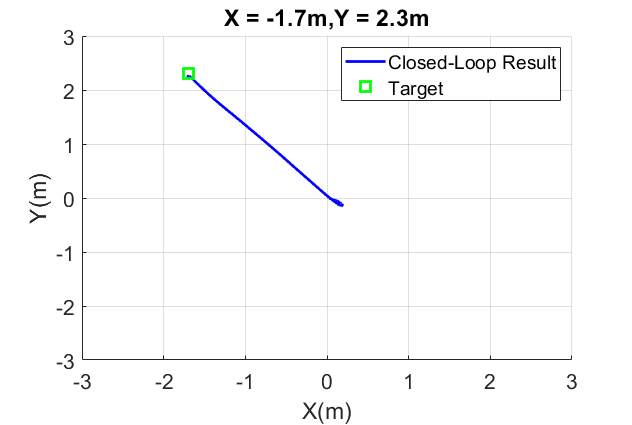
\includegraphics[width=0.9\linewidth]{images/1723closed.png}}
    \subfigure[Closed Loop Diagonal Experiment \label{fig:1723closed}]{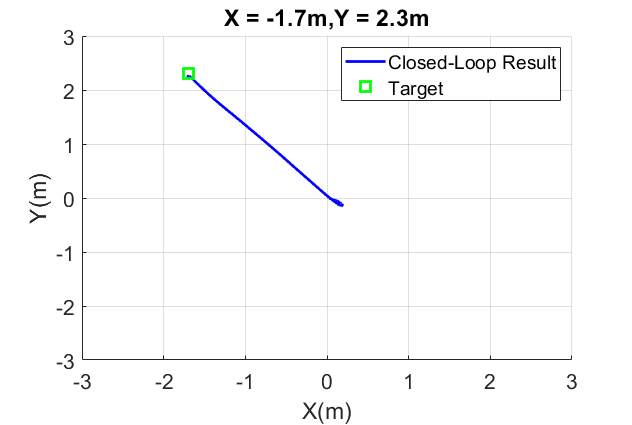
\includegraphics[width=0.9\linewidth]{images/1723closed.png}}
\end{figure}


\begin{figure}[h]
    \centering
    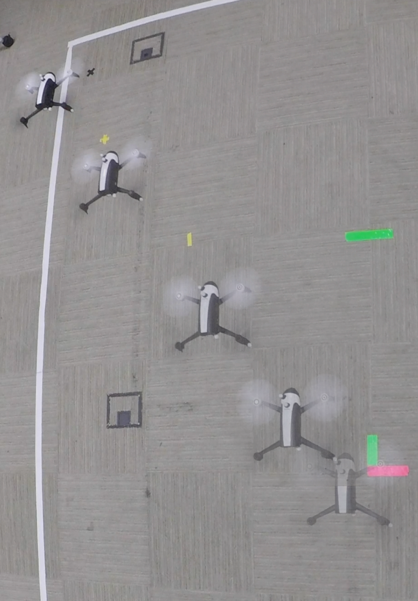
\includegraphics[width = 0.3\textwidth]{images/diagquad2.png}
    \caption{Diagonal Trajectory Experiment}
    \label{fig:diagquad}
\end{figure}
To further validate the approach, a square-shaped trajectory was tested, and the experimental data is shown in Fig.~\ref{fig:sqr}. The Parrot BeBop 2 quadrotor experiments are pictured in Fig.~\ref{fig:sqrquad}.

\begin{figure}[ht!]
	\centering
	\subfigure[Open Loop Square \label{fig:clsquare}]{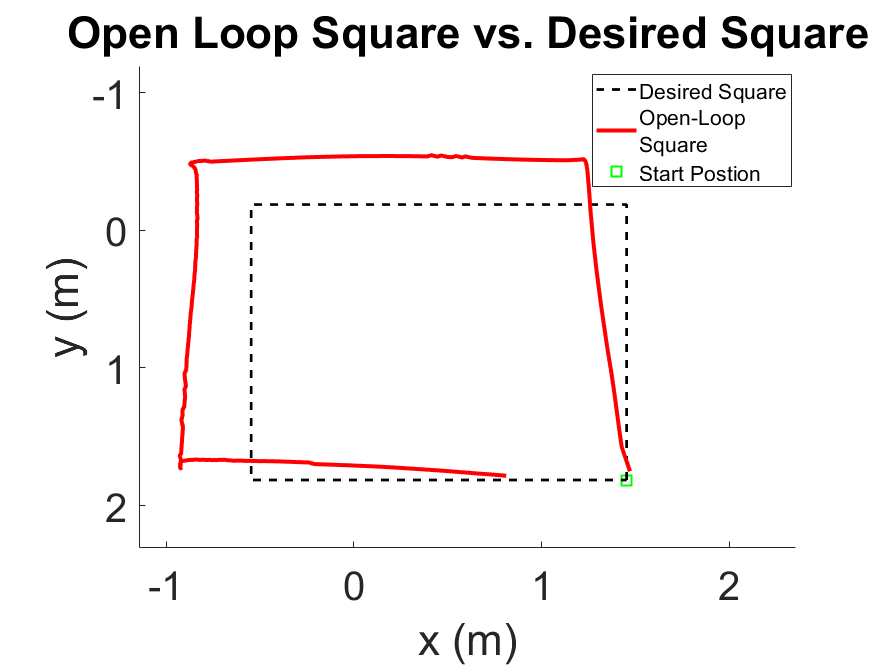
\includegraphics[width=0.48\columnwidth]{images/OPENsquare.png}}
    \subfigure[Closed Loop Square \label{fig:opensquare}]{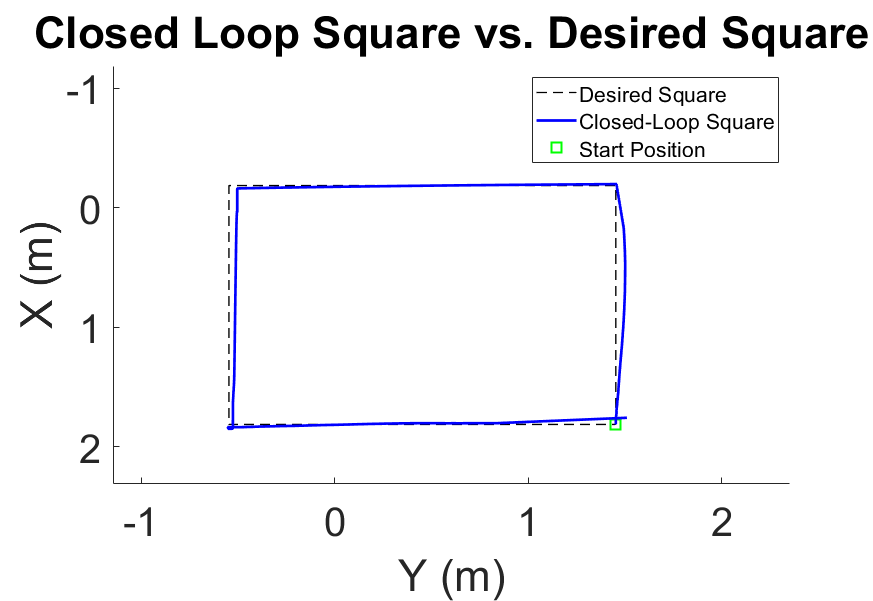
\includegraphics[width=0.48\columnwidth]{images/CLOSEDsquare.png}}
	\caption{Square-Shaped Trajectory in Open and Closed Loop}
	\label{fig:sqr}
\end{figure}

\begin{figure}[ht!]
	\centering
	\subfigure[Open Loop Square \label{fig:clsquareq}]{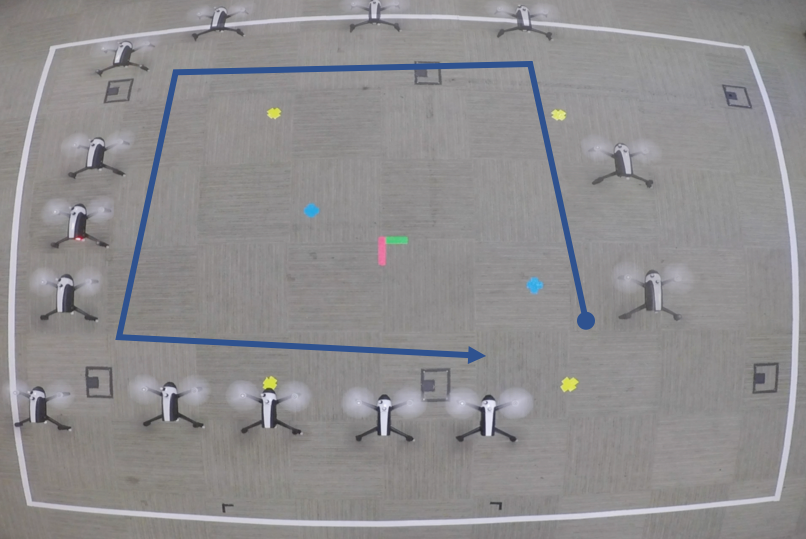
\includegraphics[width=0.48\columnwidth]{images/square_open_quad.png}}
    \subfigure[Closed Loop Square \label{fig:opensquareq}]{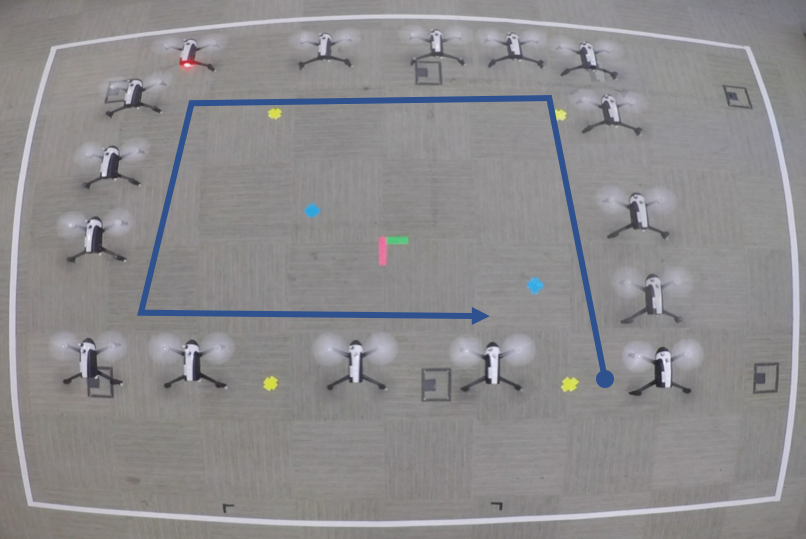
\includegraphics[width=0.48\columnwidth]{images/square_closed_quad.png}}
	\caption{Square-Shaped Trajectory Experiments}
	\label{fig:sqrquad}
\end{figure}

Lastly, the letters U, V, and A were created with the UAV. The planned trajectories were created using minimum snap trajectories and discretized, as discussed in Section~\ref{sec:traj}. The actual trajectories travelled by the UAV are shown in Fig.~\ref{fig:UVA}.

\begin{figure*}[t] \label{fig:UVA}
\subfigure[Planned U Trajectory]{\label{ex0}
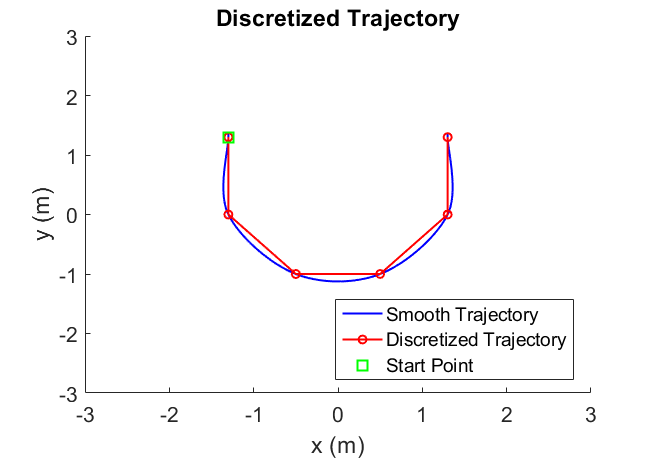
\includegraphics[width=0.3\textwidth]{images/DESIRE_U.png}}\hfill
\subfigure[Planned V Trajectory]{\label{ex1}
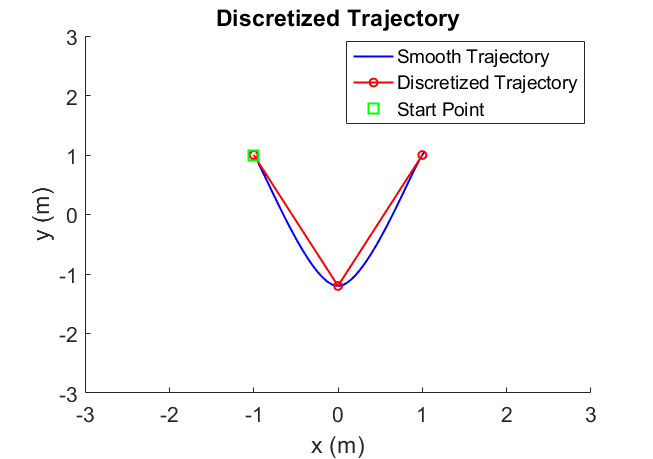
\includegraphics[width=0.3\textwidth]{images/DESIRE_V.png}}\hfill
\subfigure[Planned A Trajectory]{\label{ex3}
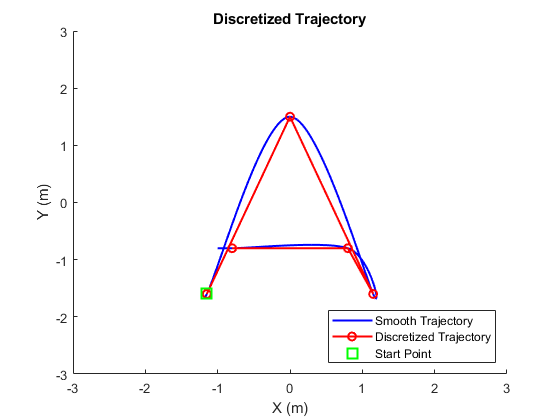
\includegraphics[width=0.3\textwidth]{images/DESIRE_A.png}}\\
\subfigure[UAV U Trajectory]{\label{ex4}
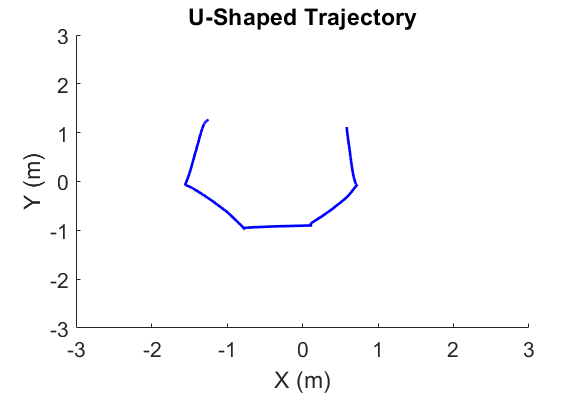
\includegraphics[width=0.3\textwidth]{images/FINAL_U.png}}\hfill
\subfigure[UAV V Trajectory]{\label{ex5}
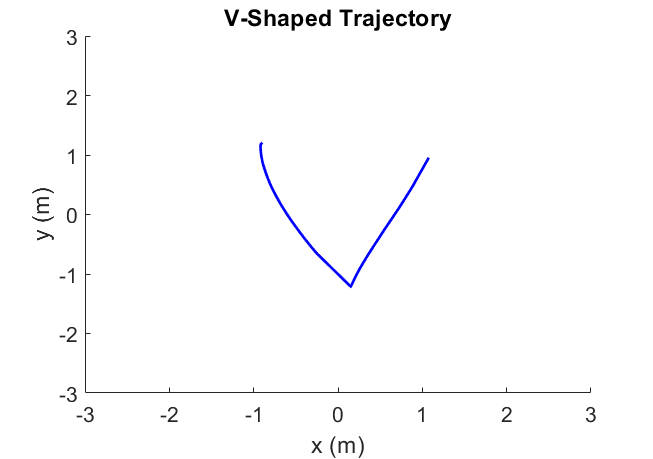
\includegraphics[width=0.3\textwidth]{images/FINAL_V.png}}\hfill
\subfigure[UAV A Trajectory]{\label{ex6}
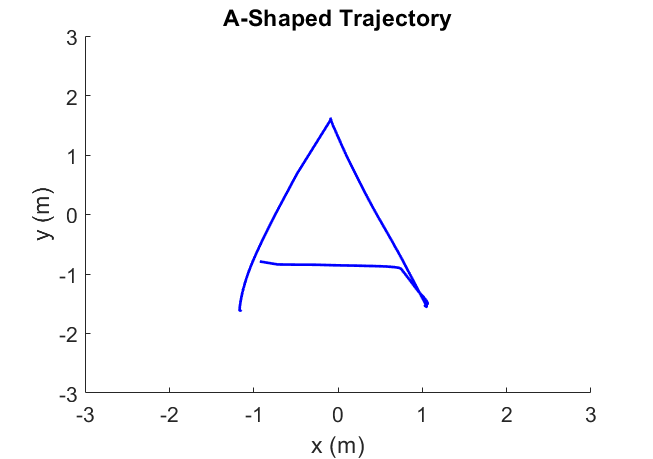
\includegraphics[width=0.3\textwidth]{images/FINAL_A.png}}\\
\end{figure*}

\section{Conclusions} \label{sec:conc}
In this work, we have presented an approach that enables autonomous flight on off-the-shelf quadrotors that are primarily tuned for teleoperation. Our approach shows that we can use a small training set along with a regression analysis to generate commands for any trajectory, along with adapting and closing the loop in real-time to reduce tracking error. Our results have shown that we are able to enable autonomous trajectory-tracking on a UAV with no knowledge of dynamic model and controller parameters. For future work, we plan to diversify some of our results by potentially using an on-board camera or IMU sensors to obtain the position of the vehicle, instead of the Vicon system. 



\section{Acknowledgement}


\addtolength{\textheight}{-12cm}   % This command serves to balance the column lengths
                                  % on the last page of the document manually. It shortens
                                  % the textheight of the last page by a suitable amount.
                                  % This command does not take effect until the next page
                                  % so it should come on the page before the last. Make
                                  % sure that you do not shorten the textheight too much.

%%%%%%%%%%%%%%%%%%%%%%%%%%%%%%%%%%%%%%%%%%%%%%%%%%%%%%%%%%%%%%%%%%%%%%%%%%%%%%%%

%References are important to the reader; therefore, each citation must be complete and correct. If at all possible, references should be commonly available publications.




\bibliographystyle{IEEEtran}
\bibliography{bib}




\end{document}
